\documentclass{article}

% \usepackage{corl_2026} % Use this for the initial submission.
% \usepackage[final]{corl_2026} % Uncomment for the camera-ready ``final'' version.
\usepackage[preprint]{corl_2026} % Uncomment for pre-prints (e.g., arxiv); This is like ``final'', but will remove the CORL footnote.

\usepackage{hyperref}       % hyperlinks
\usepackage{amsmath, amssymb, amsthm, mathtools}
\usepackage{url}            % simple URL typesetting
\usepackage{booktabs}
\usepackage{colortbl}
\usepackage{amsfonts}       % blackboard math symbols
\usepackage{graphicx}
\usepackage{multirow}
\usepackage{multicol}
\usepackage{algorithm}
\usepackage{algorithmic}
\usepackage{wrapfig}
\usepackage{subfigure}
\usepackage[most]{tcolorbox}
\usepackage{graphicx}
\usepackage{booktabs}
\usepackage{tabularx}
\usepackage{amsfonts}
\usepackage{amssymb}
\usepackage[table]{xcolor}

\definecolor{lightyellow}{RGB}{255, 247, 222}
\definecolor{reorange}{RGB}{230, 60, 0}
\definecolor{lightgray}{gray}{0.9}
\newcommand{\bz}[1]{\textcolor{blue}{[Bolei: #1]}}


\title{
  \raisebox{-.18\height}{
\includegraphics[width=0.07\textwidth]{figs/bridgesim_logo.png}}
  BridgeSim：揭示端到端自动驾驶中的开环-闭环（OL-CL）差距
}

% The \author macro works with any number of authors. There are two
% commands used to separate the names and addresses of multiple
% authors: \And and \AND.
%
% Using \And between authors leaves it to LaTeX to determine where to
% break the lines. Using \AND forces a line break at that point. So,
% if LaTeX puts 3 of 4 authors names on the first line, and the last
% on the second line, try using \AND instead of \And before the third
% author name.

% NOTE: authors will be visible only in the camera-ready and preprint versions (i.e., when using the option 'final' or 'preprint').
% 	For the initial submission the authors will be anonymized.

\author{
    Seth Z. Zhao$^1$\thanks{同等贡献。项目负责人联系方式：\texttt{sethzhao506@g.ucla.edu, luw015@ucsd.edu}.},
    Luobin Wang$^2$\footnotemark[1],
    Hongwei Ruan$^2$,
    Yuxin Bao$^1$,
    Yilan Chen$^2$,
    Ziyang Leng$^1$,
    \AND
    Abhijit Ravichandran$^2$,
    Honglin He$^1$,
    Zewei Zhou$^1$,
    Xu Han$^1$,
    Abhishek Peri$^3$,
    \AND
    Zhiyu Huang$^1$,
    Pranav Desai$^3$,
    Henrik Christensen$^2$,
    Jiaqi Ma$^1$,
    Bolei Zhou$^1$\thanks{通讯作者：\texttt{bolei@cs.ucla.edu}.} \\
    % \AND
    $^1$UCLA~~~~~~$^2$UCSD~~~~~~$^3$Qualcomm \\
    \tt{\href{https://vail-ucla.github.io/BridgeSim/}{\tt https://vail-ucla.github.io/BridgeSim/}}}



% Chinese support (auto-injected)
\usepackage{xeCJK}
\setCJKmainfont{Noto Serif CJK SC}[ItalicFont=AR PL UKai TW MBE]
\setCJKsansfont{Noto Sans CJK SC}
\setCJKmonofont{Noto Sans CJK SC}
\raggedbottom
\renewcommand{\figurename}{图}
\renewcommand{\tablename}{表}
\renewcommand{\abstractname}{摘要}
\renewcommand{\refname}{参考文献}
\begin{document}
\maketitle

%===============================================================================

\begin{abstract}
    当开环（Open-loop, OL）预训练策略在开环评估中得分很高，却无法在闭环（Closed-loop, CL）部署中有效迁移时，就存在开环到闭环差距（\textbf{OL-CL 差距}）。本文揭示了这一系统性失败的根因，并提出了切实可行的补救方案。具体而言，我们证明开环策略存在\textit{观测域偏移（Observational Domain Shift）}和\textit{目标错配（Objective Mismatch）}问题。我们表明，前者在很大程度上可通过自适应技术恢复，而后者则造成建模复杂反应式行为的结构性无能，构成OL-CL差距的主因。我们发现，大量开环策略学到有偏Q值估计器，既忽视了闭环仿真的反应式特性，也缺乏降低累积误差所需的时间感知。为此，我们提出测试时自适应（Test-Time Adaptation, TTA）框架，用于校准观测偏移、减少状态-动作偏差并强制时间一致性。大量实验表明，TTA能有效缓解规划偏差，并展现出优于基线策略的扩展动力学（scaling dynamics）。此外，我们的分析还指出，标准开环评估协议存在盲区，无法反映闭环部署的现实。

\end{abstract}

% Two or three meaningful keywords should be added here
\keywords{自动驾驶, 闭环仿真, 测试时自适应}

%===============================================================================

\section{引言}
% old intro:
% The paradigm of End-to-End ($\text{E2E}$) autonomous driving, characterized by the direct mapping of raw sensor inputs to control signals, has emerged as the prevailing architectural trend. Along this line, many recent works follow an open-loop (OL) evaluation setting on benchmarks such as nuScenes~\cite{caesar2020nuscenes} and NAVSIM~\cite{navsimv1, navsimv2} to study planning behavior, and some reporting ~\cite{RAP, DrivoR} near human-level results on these metrics. However, recent studies have unveiled a troubling discrepancy: while OL performance follows a predictable power-law relationship with data scale, this relationship breaks down during closed-loop (CL) deployment~\cite{zheng2024datascalinglaw, naumann2025datascalinglaw}. Furthermore, policies that dominate OL leaderboards often produce reactive failures or infeasible trajectories when deployed in interactive environments~\cite{jia2024bench, li2024ego, ol_cl_survey}. These observations motivate us to revisit the OL-CL gap and critically examine the limitations of current OL evaluation protocols that the community has overlooked.

% Open-loop evaluation emerged as a practical and scalable proxy for closed-loop simulation, enabling efficient benchmarking of planning policies on large-scale datasets~\cite{caesar2020nuscenes, caesar2021nuplan, navsimv1, navsimv2, li2024pretrain}, where interactive evaluation is computationally expensive and difficult to standardize~\cite{dolgov2008practical, claussmann2019review}. However, because it evaluates policies under fixed, non-reactive observations rather than sequential decision-making, strong open-loop performance may not be indicative of reliable driving behavior in closed-loop deployment~\cite{jia2024bench, li2024ego, ol_cl_survey}. This deployment gap is a composite manifestation of two distinct factors: \textit{1) Information Asymmetry}, where sensor distributions diverge between the source training domain and the target testing domain (so-called sim-to-sim gap\footnote{Here we refer the training and testing environments are different simulation environments: for example NAVSIM~\cite{navsimv1,navsimv2} is a simulation environment with real-world observations whereas Bench2Drive~\cite{jia2024bench} is a simulation environment with game-engine based observations.}), resulting in semantic information loss in the observation space; \textit{2) Objective Mismatch}, where policies optimized for OL surrogate objectives fail to align with true closed-loop returns. Through conceptual analysis (Section~\ref{section:decomposition_analysis}) and controlled experiments on our cross-simulator platform, BridgeSim (Section~\ref{section:bridgesim_platform}), we show that these factors jointly induce systematically biased Q-value estimates under closed-loop execution. Crucially, optimizing for open-loop metrics further amplifies this bias: policies are implicitly encouraged to exploit static trajectory-matching objectives via biased trajectory scorers~\cite{diffusiondrivev2}, leading to overfitting to benchmark-specific artifacts rather than learning robust, feedback-aware behaviors. As a result, the learned Q-value estimators misalign with true long-horizon returns, often producing overconfident yet brittle decisions that fail catastrophically when deployed in interactive environments.

% Based on these observations, we identify objective mismatch as the dominant and persistent source of \textit{OL-to-CL} degradation. While information asymmetry can often be mitigated through observation calibration, the bias in Q-value estimation induced by OL training fundamentally limits deployment performance, and is further exacerbated by horizon misalignment between training and execution. To address this, we propose a plug-and-play test-time adaptation (TTA) framework that enables OL-pretrained policies to operate robustly in closed-loop settings without retraining. Our framework consists of three components: 1) \textit{Flow-matching-based Observational Calibrator} for cross-domain feature alignment; 2) \textit{Unbiased Q-value Estimator} that corrects the scoring bias introduced during OL training; and 3) \textit{Adaptive Replan Mechanism} for reactive decision-making under evolving dynamics. Extensive experiments demonstrate that our approach improves closed-loop performance by up to 50\% across diverse scenario conditions. Furthermore, our experiments reveal a more favorable scaling dynamics of OL policies under the TTA framework compared with baselines. Based on these findings, we suggest the community reassess the prevailing reliance on non-reactive open-loop evaluations and move toward closed-loop-aligned training objectives and evaluation protocols that account for the interactive nature of real-world driving. There are key contributions as follows:

端到端（End-to-End, E2E）自动驾驶领域有越来越多的工作致力于在开环（OL）基准（benchmark）上取得高分，如 nuScenes~\cite{caesar2020nuscenes} 和 NAVSIM~\cite{navsimv2, navsimv1}，其中一些方法报告了接近甚至达到人类水平的性能~\cite{RAP, DrivoR}。然而，开环策略输出的轨迹在闭环（CL）仿真部署中常常变得不可行或不安全，与其在开环评估中所声称的表现存在显著差异~\cite{jia2024bench, li2024ego, ol_cl_survey,zhao2025quantv2x}。本文将这种差异称为端到端驾驶中的\textbf{OL-CL 差距}。

揭示OL-CL差距对于避免从开环基准中得出虚幻结论至关重要。我们在图~\ref{fig:bridgesim_hero} 中说明动机。首先，开环基准上的成功可能成为现实条件下驾驶行为的一个误导性代理指标。近期工作~\cite{jia2024bench, li2024ego, ol_cl_survey} 已证明在相似的域设置下，开环与闭环性能之间缺乏对应关系；而且随着仿真时域的增加，这种相关性进一步衰减（见图~\ref{fig:empirical_objective_mismatch}）。其次，开环规模定律（scaling law）无法预测闭环扩展：近期研究表明，开环性能随数据量和测试时算力呈可预测的扩展关系，但这两者都无法可靠地迁移到闭环部署~\cite{zheng2024datascalinglaw, naumann2025datascalinglaw}。这些差异表明，开环评估协议虽是代价高昂的闭环仿真的实用且可扩展的代理指标~\cite{caesar2020nuscenes, caesar2021nuplan, navsimv1, navsimv2, li2024pretrain}，但可能存在偏差，并忽视了现实世界驾驶策略应当优化的根本目标。

\begin{figure}[tbh]
    \centering
    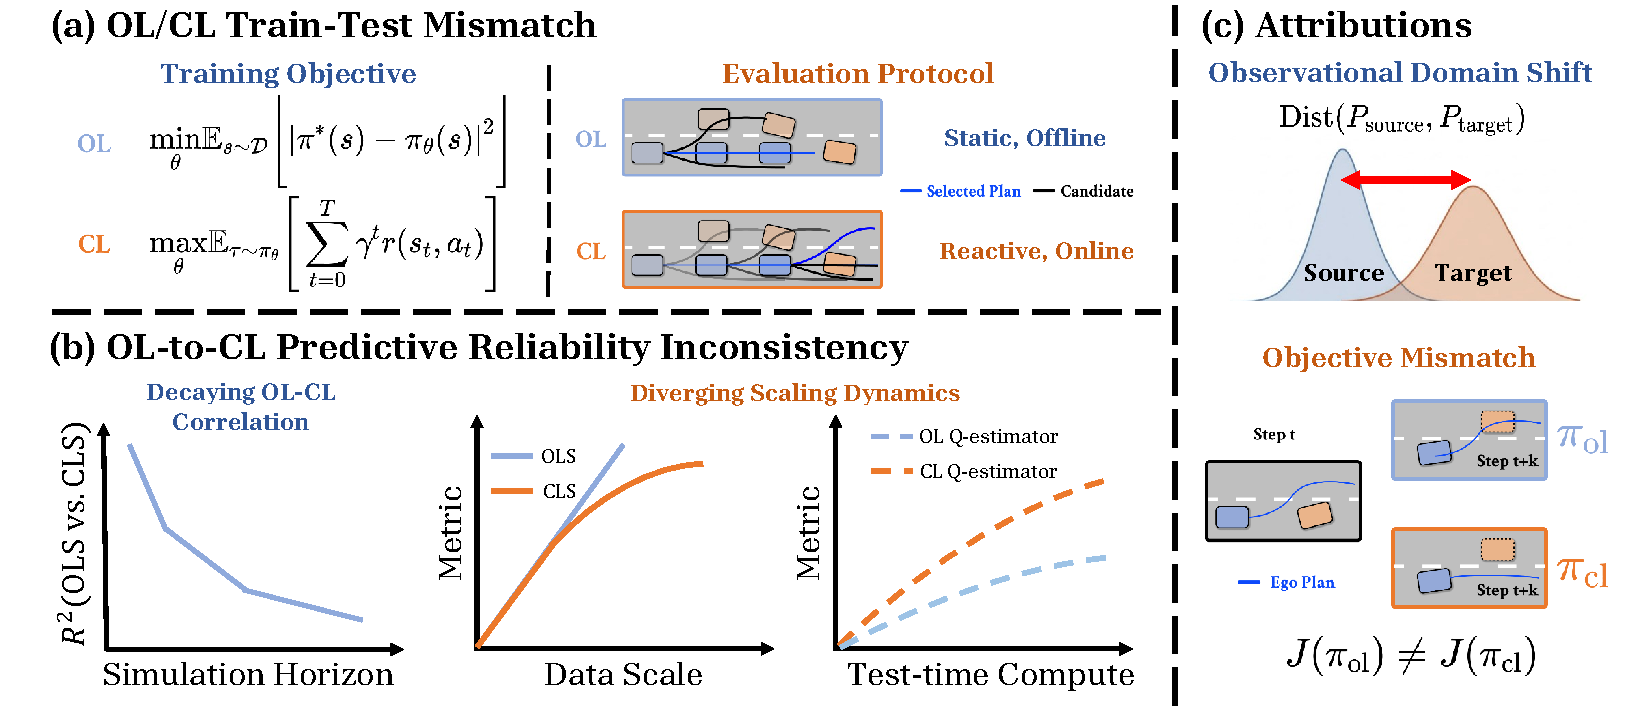
\includegraphics[width=.99\linewidth]{figs/bridgesim_hero.pdf}
    \vspace{-1em}
    \caption{\textbf{动机。} \textbf{(a)}：开环（OL）训练-测试范式未必与闭环（CL）部署的目标和评估指标一致；\textbf{(b)}：这种错配导致显著的性能差异，表现为相关性衰减与扩展动力学（scaling dynamics）发散；\textbf{(c)}：我们将这种OL-CL差距归因于\textit{观测域偏移}与\textit{目标错配}。}
    \label{fig:bridgesim_hero}
    \vspace{-2em}
\end{figure}

本文的目的并非批评开环评估协议或源自开环评估的方法开发，而是澄清策略\textit{可能在何处}失败，以及需要\textit{何种}自适应手段来缓解闭环部署中的失败。本文的主要贡献总结如下：

\textbf{1. 识别端到端自动驾驶中OL-CL差距的根本失效模式}。我们将OL-CL差距追溯到两个不同来源。其一是\textit{观测域偏移}，即测试时的传感器观测与训练时所见不同。这种分布偏移在规划尚未开始之前就损害了感知（即所谓的仿真间差距（sim-to-sim）\footnote{这里我们指训练与测试环境是不同的仿真环境：例如，NAVSIM~\cite{navsimv1,navsimv2} 是使用真实世界观测的仿真环境，而 Bench2Drive~\cite{jia2024bench} 是基于游戏引擎观测的仿真环境。}~\cite{garcia2025road}）。虽然我们的研究强调域自适应可以恢复大部分丢失的感知保真度，但仅解决域差距并不能\textit{防止}闭环失败。第二个也是更根本的来源，是开环训练与闭环测试之间的\textit{目标错配}。更具体地说，开环训练优化的是静态轨迹匹配目标，并不对应真实的闭环回报，由此产生的Q值估计存在偏差，并过拟合于预训练仿真器。这种偏差是结构性的，无论感知输入校准得多么好都会持续存在。

\textbf{2. 提出缓解闭环部署失败的测试时自适应（TTA）框架}。该框架包含一个\textit{基于流匹配的观测校准器}，用于在训练环境与部署环境之间进行跨域观测对齐；以及一个\textit{免训练的自适应机制}，用于解决结构性错配。具体而言，我们通过\textit{截断Q值估计器}适配开环策略，以纠正开环训练目标引入的评分偏差；\textit{自适应重规划机制}使策略能够在环境动力学演化时进行反应式重规划。这些组件共同缓解了上述开环到闭环的部署失败。在闭环仿真的多样场景中，我们的方法在基线方法的基础上将闭环性能提升最高22\%，并展现出比基线策略更有利的扩展行为。

\textbf{3. 提出BridgeSim——一个跨仿真器端到端闭环仿真平台}。为补充现有端到端基准，我们开发了一个综合性平台，用于在交互式、闭环设置下对任意端到端驾驶策略进行严谨、动态的评估。

\section{相关工作}
\textbf{驾驶仿真器与基准测试。}驾驶仿真器与基准测试很早就被认为是训练和评估自动驾驶系统的关键工具，为算法开发提供了安全、高效且可重复的环境~\cite{alghodhaifi2021autonomous, rosique2019systematic, ye2019automated, osinski2020simulation, wu2024recent}。GTA V~\cite{gtav}、Sim4CV~\cite{muller2018sim4cv}、AIRSIM~\cite{shah2018airsim} 和 CARLA~\cite{dosovitskiy2017carla} 等各类传统游戏引擎仿真器和高保真仿真器提供可配置的环境和复杂的物理条件建模。同样，DeepDrive~\cite{deepdrive} 和 DriverGym~\cite{kothari2021drivergym} 等轻量级平台提供简化的动力学以支持快速实验，而 MetaDrive~\cite{li2022metadrive} 等仿真器则专注于模块化、可扩展性以及多智能体交互丰富的场景。尽管这些传统平台有其实用价值，但由于手工制作的资产和有限的视觉真实感，它们常常存在域差距。近期的努力探索了数据驱动和生成式仿真框架来弥合这一差距。DriveArena~\cite{yang2024drivearena} 合成逼真的交通场景，以促进迭代的感知-动作循环。HUGSIM~\cite{zhou2024hugsim} 和 RAD~\cite{gao2025rad} 利用3D高斯泼溅（3D Gaussian Splatting）进行实时、照片级逼真的场景重建和闭环仿真，进一步推进了这一方向。此外，ReconDreamer 和 ReconDreamer-RL~\cite{ni2025recondreamer, ni2025recondreamerrl} 展示了基于世界模型的重建框架，以解决新轨迹表征方面的局限。然而，现有生成式仿真框架仍存在仿真伪影，并缺乏评估端到端策略所需的指标标注（见附录~\ref{appendix:current_e2e_bottlenecks}）。

\textbf{端到端自动驾驶。}传统自动驾驶系统采用由感知、预测和规划模块组成的模块化设计，但这些模块存在误差传播和信息丢失问题~\cite{luo2018fast, liang2020pnpnet, sadat2020perceive, li2024womd}。随后，近期研究转向将原始传感器输入直接映射到控制命令的集成式端到端（E2E）范式。UniAD~\cite{uniad} 将各模块集成到统一框架中，并利用栅格化表征进行信息传递。VAD~\cite{vad} 用实例中心的向量化表征替代稠密栅格，进一步优化了效率；TransFuser~\cite{transfuser} 则将输入扩展到多模态。近期，DiffusionDrive 和 DiffusionDriveV2~\cite{diffusiondrive, diffusiondrivev2} 通过扩散策略对动作的多模态分布进行建模。DrivoR~\cite{DrivoR} 利用寄存器令牌避免复杂的中间表征，同时保持优越的性能。
尽管规划评估指标的性能有所提升，但 AD-MLP、PDM-Close、BEV-Planner、LEAD 和 RAP~\cite{zhai2023rethinking, dauner2023parting, li2024ego, LEAD, RAP} 等近期工作指出了开环（OL）基准的局限，并揭示了弥合OL-CL差距的必要性。虽然对端到端策略进行闭环（CL）训练可以缓解这一差距，但会带来更高的复杂度和计算成本~\cite{KarkusBeyondBC}。相反，本文工作将端到端驾驶中的OL-CL差距归因于两个不同因素，并提出通过测试时自适应来弥合这一差距。

\begin{table}[tbh]
\centering
\caption{与其他E2E开环和闭环基准的对比。MV-Consistency：多视图时间一致性，TF-Consistency：交通元素标注一致性。PG：程序化地图与行为生成。关于BridgeSim平台的更多细节见附录~\ref{appendix:bridgesim_platform}。}
\label{tab:benchmark_comparison}
\resizebox{\textwidth}{!}{
    \begin{tabular}{l|cccccc}
    \toprule
    \textbf{名称} & \textbf{闭环} & \textbf{长期仿真} & \textbf{MV-Consistency} & \textbf{TF-Consistency} & \textbf{支持的地图} & \textbf{支持的交通模式} \\
    \midrule
    NAVSIM~\cite{navsimv1, navsimv2}           & $\times$ & $\times$ & \checkmark & \checkmark & nuPlan & Log-replay \\
    Bench2Drive~\cite{jia2024bench}  & \checkmark & \checkmark & \checkmark & \checkmark & CARLA & IDM \\
    DriveArena~\cite{yang2024drivearena} & \checkmark & \checkmark & $\times$ & $\times$ & nuScenes & Log-replay \\
    HUGSIM~\cite{zhou2024hugsim}     & \checkmark & \checkmark & \checkmark & $\times$ &  nuScenes, Waymo, KITTI-360, PandaSet & Log-replay, IDM, Adversarial \\
    \midrule
    \textbf{BridgeSim (ours)}        & \checkmark & \checkmark & \checkmark & \checkmark &  CARLA, Waymo, nuScenes, nuPlan, PG & Log-replay, IDM, Adversarial \\
    \bottomrule
    \end{tabular}
}
\end{table}

\section{BridgeSim：用于E2E驾驶策略的统一跨仿真器闭环仿真平台}
\label{section:bridgesim_platform}

为以可量化的严谨性实证研究OL-CL差距，我们提出BridgeSim——一个跨仿真器平台，用于在高保真闭环环境中评估开环预训练策略。BridgeSim设计统一的场景协议，将多样的地图场景（如 nuPlan~\cite{caesar2021nuplan}、WOMD~\cite{mei2022waymo} 和 nuScenes~\cite{caesar2020nuscenes}）与异构的交通模式（如日志回放（Log-replay）、智能驾驶员模型（Intelligent Driver Model, IDM）~\cite{idm} 和对抗性策略~\cite{advbmt}）相结合，以在闭环仿真环境中对端到端驾驶策略进行压力测试。此外，BridgeSim提供灵活的部署设置，能以不同的执行频率和仿真时域模拟开环策略。因此，BridgeSim弥合了局限于短期静态预测的开环基准与现有往往缺乏复杂反应式压力测试所需综合功能和标注的闭环基准之间的关键鸿沟。表~\ref{tab:benchmark_comparison} 给出了BridgeSim与其他主流E2E基准的全面功能对比。

\section{分解开环到闭环（OL-CL）差距}
\label{section:decomposition_analysis}
本节中，我们重新审视端到端驾驶任务的理论形式化，并分析OL-CL差距的失效模式，即\textit{观测域偏移}和\textit{目标错配}。通过实证研究，我们进一步说明这些因素导致的性能下降，从而启发测试时自适应框架的设计，使开环策略从失败中恢复。

\subsection{预备知识与记号}
\label{subsec:preliminaries}
\noindent \textbf{POMDP形式化。}我们将端到端驾驶任务形式化为部分可观测马尔可夫决策过程（Partially Observable Markov Decision Process, POMDP），由元组 $\langle \mathcal{S}, \mathcal{A}, \mathcal{O}, \mathcal{T}, \Omega, r, \gamma, \rho_0, T \rangle$ 定义。其中 $\mathcal{S}$ 表示环境的真实底层状态空间，$\mathcal{A}$ 是自车的动作空间，$\mathcal{O}$ 是高维观测空间。在时间步 $t$，系统处于状态 $s_t \in \mathcal{S}$。智能体接收由发射分布 $\Omega(o_t \mid s_t)$ 支配的观测 $o_t \in \mathcal{O}$，执行动作 $a_t \in \mathcal{A}$，环境通过 $\mathcal{T}(s_{t+1} \mid s_t, a_t)$ 演化。回合在有限时域 $T$ 步内进行，其中 $\rho_0(s_0)$ 表示初始状态分布，$\gamma \in [0, 1)$ 为折扣因子。

% \textbf{E2E Driving Policy.} Recent E2E policies~\cite{diffusiondrive, diffusiondrivev2, RAP} are  governed by a stochastic policy parameterized by an observation encoder $\theta$ (e.g., a pretrained vision encoder) and an action decoder $\phi$ (e.g., a control head). We formulate these state-conditioned policies as $\pi^{\Omega}_{\theta, \phi}(a_{t:t+H} \mid s)$, where the agent interacts with the underlying state exclusively through the observation channel $\Omega$. This notation explicitly isolates the dependence of the agent's behavior on the environment's emission model. Concretely, we consider an encoder $f_\theta:\mathcal{O}\to\mathcal{Z}$ that maps raw observations to a latent scene representation $z\in\mathcal{Z}$, followed by a policy head $\pi_\phi(a\mid z)$ that outputs the trajectory-action. Thus, we could define the joint distribution of E2E driving policy as isolated components over $(a,z,o)$ conditioned on state $s$:
\noindent \textbf{端到端驾驶策略。}我们考虑由随机映射 $\pi^{d}_{\theta,\phi}$ 表示的端到端（E2E）驾驶策略，该映射由观测域 $d\in\{\mathrm{source},\mathrm{target}\}$、观测编码器参数 $\theta$ 和行为解码器参数 $\phi$ 参数化。我们考虑预测动作序列 $\mathbf{a}_t\in\mathcal{A}$\footnote{我们用粗体字符 $\mathbf{a}_t$ 表示一段控制序列 $a_{t:t+H}$。$H$ 是训练阶段确定的固定预测序列长度。}的策略。智能体通过依赖域的发射分布 $\Omega^d(o_t\mid s_t)$ 接收底层环境状态 $s_t\in S$ 的观测 $o_t\in \mathcal{O}$。该设定使我们能够将观测域偏移与行为域偏移分离开来。具体而言，编码器 $f_\theta: \mathcal{O} \to \mathcal{Z}$ 将原始观测映射为潜在场景表征 $z \in \mathcal{Z}$，而策略头 $\pi_\phi(\mathbf{a}_t \mid z_t)$ 生成自车的未来轨迹。端到端策略的联合分布随后可在状态 $s_t$ 条件下分解为动作序列、潜在表征和观测 $(\mathbf{a}_t, z_t, o_t)$ 上的分量：
\begin{equation}
%\small
\label{eq:policy_state_latent_factor}
    \pi^{d}_{\theta,\phi}(\mathbf{a}_t,z_t,o_t \mid s_t) \triangleq \pi_{\phi}(\mathbf{a}_t\mid z_t)\,P_\theta(z_t\mid o_t)\,\Omega^d(o_t\mid s_t),
\end{equation}
其中 $P_\theta(z_t\mid o_t)$ 表示编码器诱导的条件分布。近期工作~\cite{diffusiondrive, diffusiondrivev2, RAP} 通常使用确定性编码器 $z_t=f_\theta(o_t)$，因此可写作 $P_\theta(z_t\mid o_t)=\delta(z_t-f_\theta(o_t))$。

% \textbf{Closed-loop Simulation, Closed-loop Execution, and Trajectory-Action Space.} We define the expected closed-loop cumulative return of a policy $\pi$ as follows:
% % \begin{equation}
% %     R_k(s_t, a_t) \triangleq \sum_{\tau=0}^{k} \gamma^\tau r(\hat{s}_{t+\tau}, u_{t+\tau}),
% % \end{equation}
% \begin{equation}
%     \label{eq:closed_loop_return_objective}
%     J(\pi) \triangleq \mathbb{E}_{s_0 \sim \rho_0} [V^\pi(s_0)] = \mathbb{E}_{s_0 \sim \rho_0,\tau \sim \pi} \left[ \sum_{t=0}^{T} \gamma^{t} r(s_t, a_t) \right]
%     % =\mathbb{E}_{s_0 \sim \rho_0,\tau \sim \pi} \left[ \sum_{t=0}^{T/k} \gamma^{t*k} \sum_{i=0}^{k} \gamma^i r(s_{t+i}, a_{t+i}) \right],
% \end{equation}


% But most of the work is optimizing
% \begin{equation}
%     \label{eq:closed_loop_return_objective}
%     J_k(\pi) =\mathbb{E}_{s_0 \sim \rho_0,\tau \sim \pi_k} \left[ \sum_{t=0}^{T/k} \gamma^{t*k} \sum_{i=0}^{k} \gamma^i r(s_{t+i}, a_{t+i}) \right],
% \end{equation}


% where $r(s_t, a_t)$ denotes the reward function and $T$ denotes the simulation horizon. The closed-loop objective of driving agent is to find a policy $\pi^*$ that maximizes the expected cumulative return.
% To enforce temporal consistency in planning over a horizon $H$, we define the action $a_t$ as a sequence of continuous primitive controls:$a_t \triangleq \{u_{t+\tau}\}_{\tau=0}^{H-1} \in \mathcal{A} \subseteq \mathcal{U}^H$, where $\mathcal{U} \subset \mathbb{R}^{d_u}$ represents the primitive control space.
% In closed-loop execution, we formalize control via a receding horizon framework. At step $t$, the policy samples a full trajectory $a_{t:t+H} \sim \pi^{\Omega}_{\theta, \phi}(\cdot \mid s_t)$, but executes only a prefix of $k$ primitive controls $\{a_{t+i}\}_{i=0}^{k-1}$, where $1 \le k \le H$ denotes the replanning horizon. Following execution, the environment advances to $t+k$, a new observation is emitted, and the planning cycle repeats.
\noindent \textbf{闭环目标。}我们通过期望闭环累积回报 $J(\pi) \triangleq \mathbb{E}_{s_0 \sim \rho_0, \tau \sim \pi} \left[ \sum_{t=0}^{T} \gamma^{t} r(s_t, a_t) \right]$ 最大化驾驶策略 $\pi$ 的性能，其中奖励函数 $r(s_t, a_t)$ 评估\textit{实际执行}的控制 $a_t$，它通常只是策略在每个时间步生成的全序列 $a_{t:t+H}$ 的部分子集。

% \textbf{KL-Regularized RL Fine-Tuning.}
% We define the reinforcement learning fine-tuning objective to maximize the expected reward while penalizing deviations from a reference policy. Adapting to our established state-action formulation, the objective is defined as the following maximization problem over the policy parameters:
% \begin{equation}
%     \max_{\theta, \phi} \mathbb{E}_{s \sim \rho(s)} \left[ \mathbb{E}_{a \sim \pi^{\Omega}_{\theta, \phi}(\cdot \mid s)} [r(s, a)] - \beta D_{\mathrm{KL}} \left( \pi^{\Omega}_{\theta, \phi}(\cdot \mid s) \parallel \pi_{\mathrm{ref}}(\cdot \mid s) \right) \right],
% \end{equation}
% where $\rho(s)$ denotes the state sampling distribution. Depending on the fine-tuning protocol, $\rho(s)$ may correspond to the expert's state distribution from the offline dataset $d^{\pi^\star}$, or the policy's induced closed-loop distribution $d^{\pi_{\theta, \phi}}$. Here, $\pi_{\mathrm{ref}}$ is a fixed reference policy (e.g., the pre-trained behavioral cloning prior), and $\beta > 0$ is the regularization coefficient. The Kullback-Leibler divergence over the trajectory-action space is formally defined as:
% \begin{equation}
%     D_{\mathrm{KL}}(q(\cdot \mid s) \parallel p(\cdot \mid s)) \triangleq \mathbb{E}_{a \sim q(\cdot \mid s)} \left[ \log \frac{q(a \mid s)}{p(a \mid s)} \right].
% \end{equation}

% \begin{figure}[tbh]
%     \centering
%     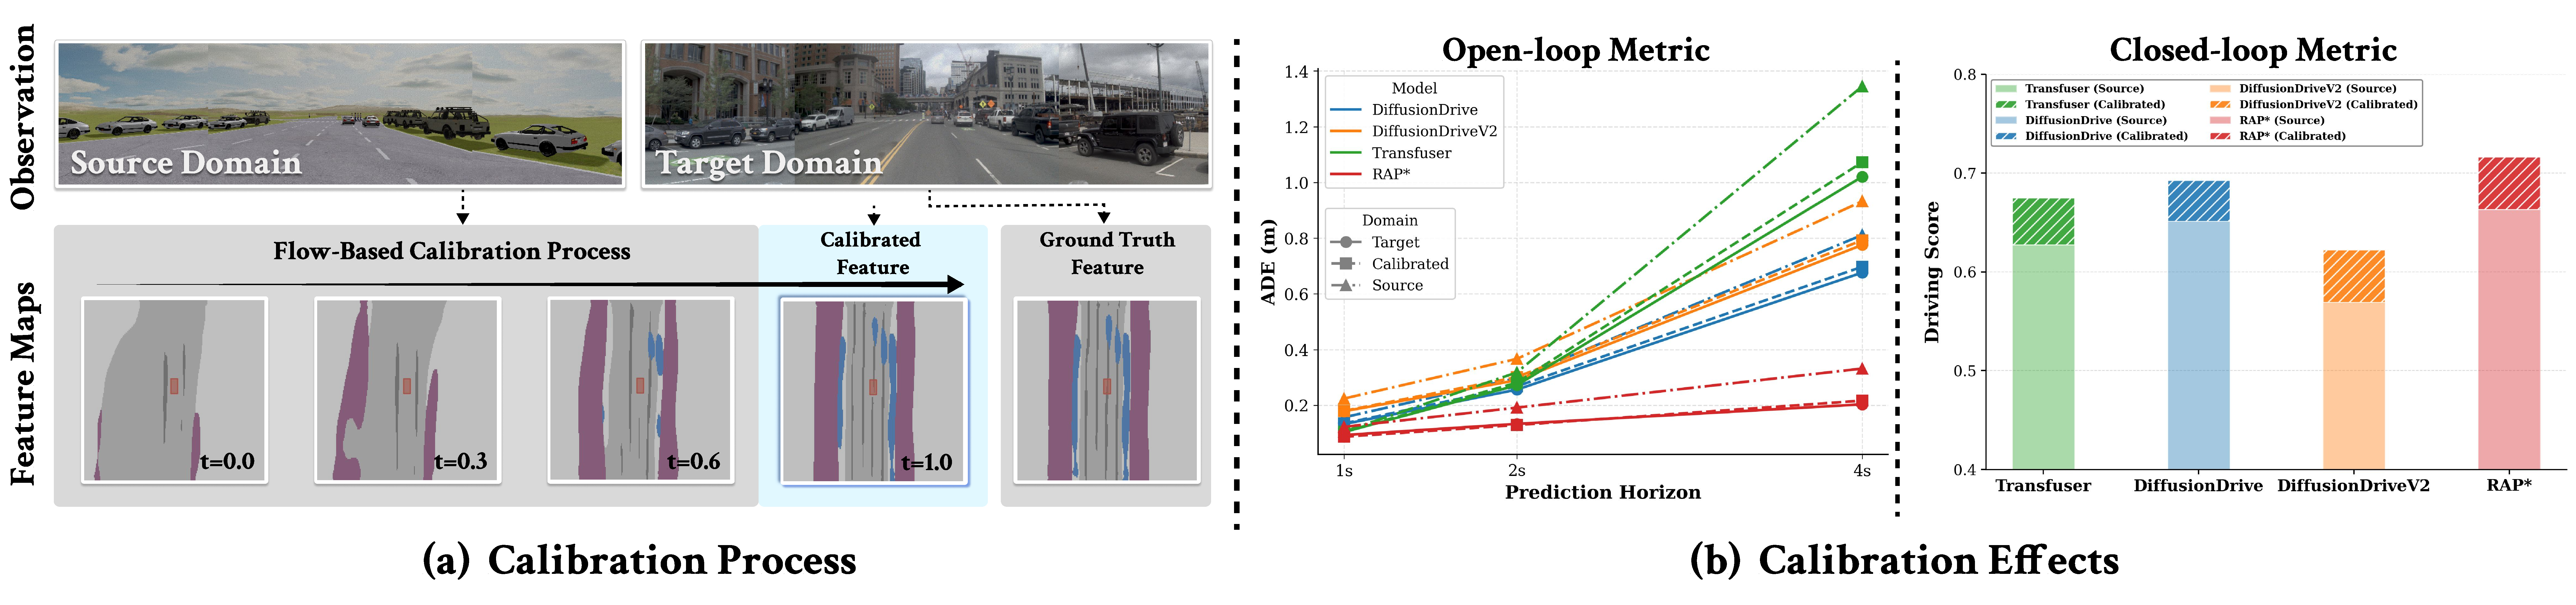
\includegraphics[width=0.99\linewidth]{figs/3.2_empirical.pdf}
%     \caption{\textbf{Empirical Study on Information Asymmetry.} a) Standard observational encoders often fail to extract salient features when deployed in new domains, leading to a significant degradation in downstream policy performance. b) Calibration effect on closed-loop performance.}
%     \label{fig:empirical_information_asymmetry}
% \end{figure}

\subsection{观测域偏移}
\label{subsec:observational_shift}
\textbf{失效模式分析。}当观测编码器无法在目标环境中提取一致的语义特征（如车道、目标等），从而损害规划所需的\textit{状态可观测性}时，就会发生观测域偏移，如图~\ref{fig:empirical_observational_shift}(a) 所示。为刻画该域偏移对任务性能的影响，我们将\emph{观测域差距（Observational Domain Gap）} $\Delta_{\mathrm{obs}}$ 定义为：
\begin{equation}
\small
    \Delta_{\mathrm{obs}}(\theta, \phi) \triangleq J(\pi^{\mathrm{source}}_{\theta,\phi}) - J(\pi^{\mathrm{target}}_{\theta,\phi}),
\end{equation}
其中相同的控制头 $\pi_\phi$ 将期望回报的下降隔离为仅由域偏移导致的部分。源域与目标域之间的差异可通过下式度量：
\begin{equation}
\small
    \label{eq:observation_gap}
    \mathrm{Dist}_Z(s;\theta) \triangleq \mathrm{Dist}\!\Big( P_\theta(z\mid o)\,\Omega^{\mathrm{source}}(o\mid s),\; P_\theta(z\mid o)\,\Omega^{\mathrm{target}}(o\mid s) \Big),
\end{equation}
其中 $\mathrm{Dist}(\cdot,\cdot)$ 是 $\mathcal{Z}$ 上分布的距离度量。基于这一形式化，我们假设只要校准观测编码器 $\theta$ 以最小化分布距离，观测域差距就是可恢复的。

\begin{figure}[tbh]
    \centering
    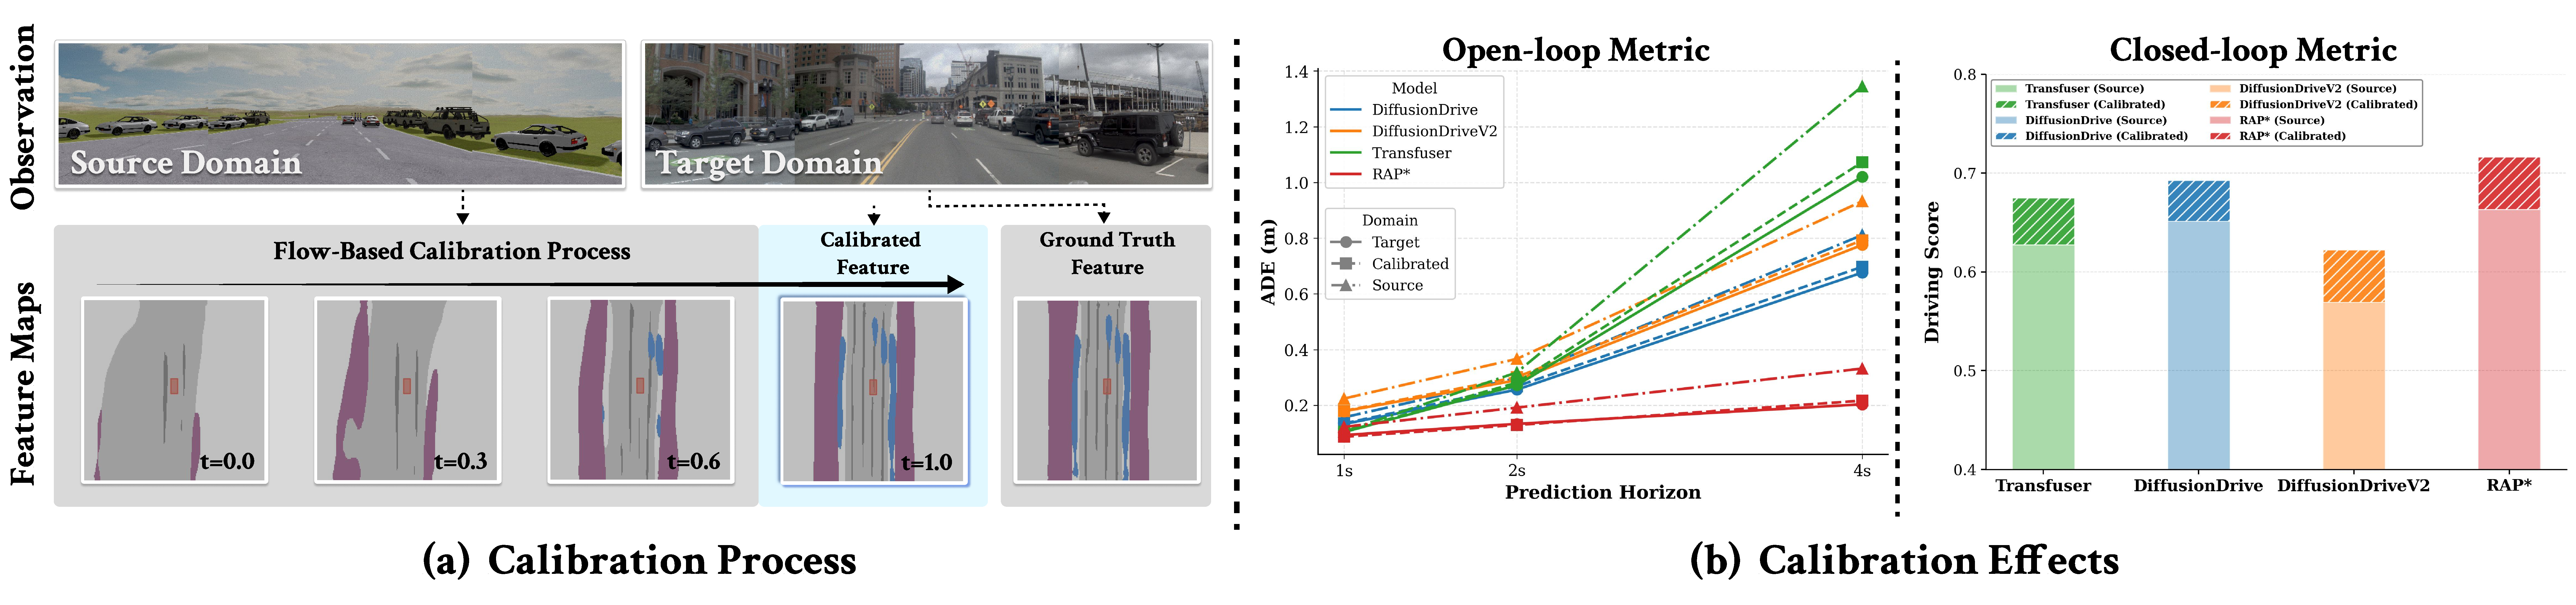
\includegraphics[width=.99\linewidth]{figs/3.2_empirical.pdf}
    \vspace{-1em}
    \caption{\textbf{观测域偏移的实证研究。} \textbf{(a)}：观测校准的流匹配（Flow-matching）过程；\textbf{(b)}：校准对开环和闭环指标的影响。实验细节见附录~\ref{appendix:observational_shift_details}。}
    \label{fig:empirical_observational_shift}
    \vspace{-2em}
\end{figure}

\textbf{实证研究。}为检验这一假设，我们隔离并量化 $\Delta_{\mathrm{obs}}$，以考察观测域偏移下的策略行为，如图~\ref{fig:empirical_observational_shift}(b) 所示。为将观测误差与闭环动力学的累积效应（如控制漂移）明确解耦，我们进行了开环消融研究。在保持底层状态转移不变、仅改变输入观测域的条件下，我们按照~\cite{lin2025modelbased} 中的协议度量轨迹相对专家真值的偏离。我们发现，在观测偏移下，由于感知模块无法提取规划所需的语义信息，策略性能急剧下降。然而，应用我们的实用校准方法（第~\ref{subsec:observational_calibrator}~节）可以成功恢复这些场景特征并最小化差距。这些结果表明：\textbf{尽管观测域偏移在规划之前就损害了感知，但这对于驾驶策略而言在很大程度上是一种可恢复的失败，针对性的校准可以有效恢复其状态可观测性并弥合域差距。}

\subsection{目标错配}
\label{subsec:objective_mismatch}
\textbf{失效模式分析。}目标错配发生在开环策略的训练目标优化\textit{静态全序列目标}、而忽视了测试时闭环部署中\textit{反应式、滚动时域的现实}时：智能体预测长度为 $H$ 的轨迹，但只执行前 $k$ 步的短前缀，然后接收新的观测并执行重规划。在实际闭环仿真中，由执行时域 $k$ 参数化的\textbf{统一闭环目标}\footnote{我们重申该公式以强调执行时域 $k$ 在闭环仿真中的重要性。注意，第~\ref{subsec:preliminaries}~节定义的标准闭环目标在 $k=1$ 时是公式~\ref{eq:executed_closed_loop_return_objective} 的特例。}定义如下：
\begin{equation}
\small
\label{eq:executed_closed_loop_return_objective}
    J_k(\pi) = \mathbb{E}_{s_0 \sim \rho_0, \tau \sim \pi_k} \left[ \sum_{c=0}^{T/k - 1} \gamma^{c \cdot k} \sum_{i=0}^{k-1} \gamma^i r(s_{c \cdot k + i}, a_{c \cdot k + i}) \right],
\end{equation}
其中 $\pi_k$ 表示以 $1/k$ 的频率执行重规划的策略，$c$ 表示规划周期。该公式使我们能够从两个维度分解目标错配带来的\textit{开环到闭环}性能下降，即\textbf{有偏的Q值估计}和\textbf{累积执行误差}。

\begin{figure}[tbh]
    \centering
    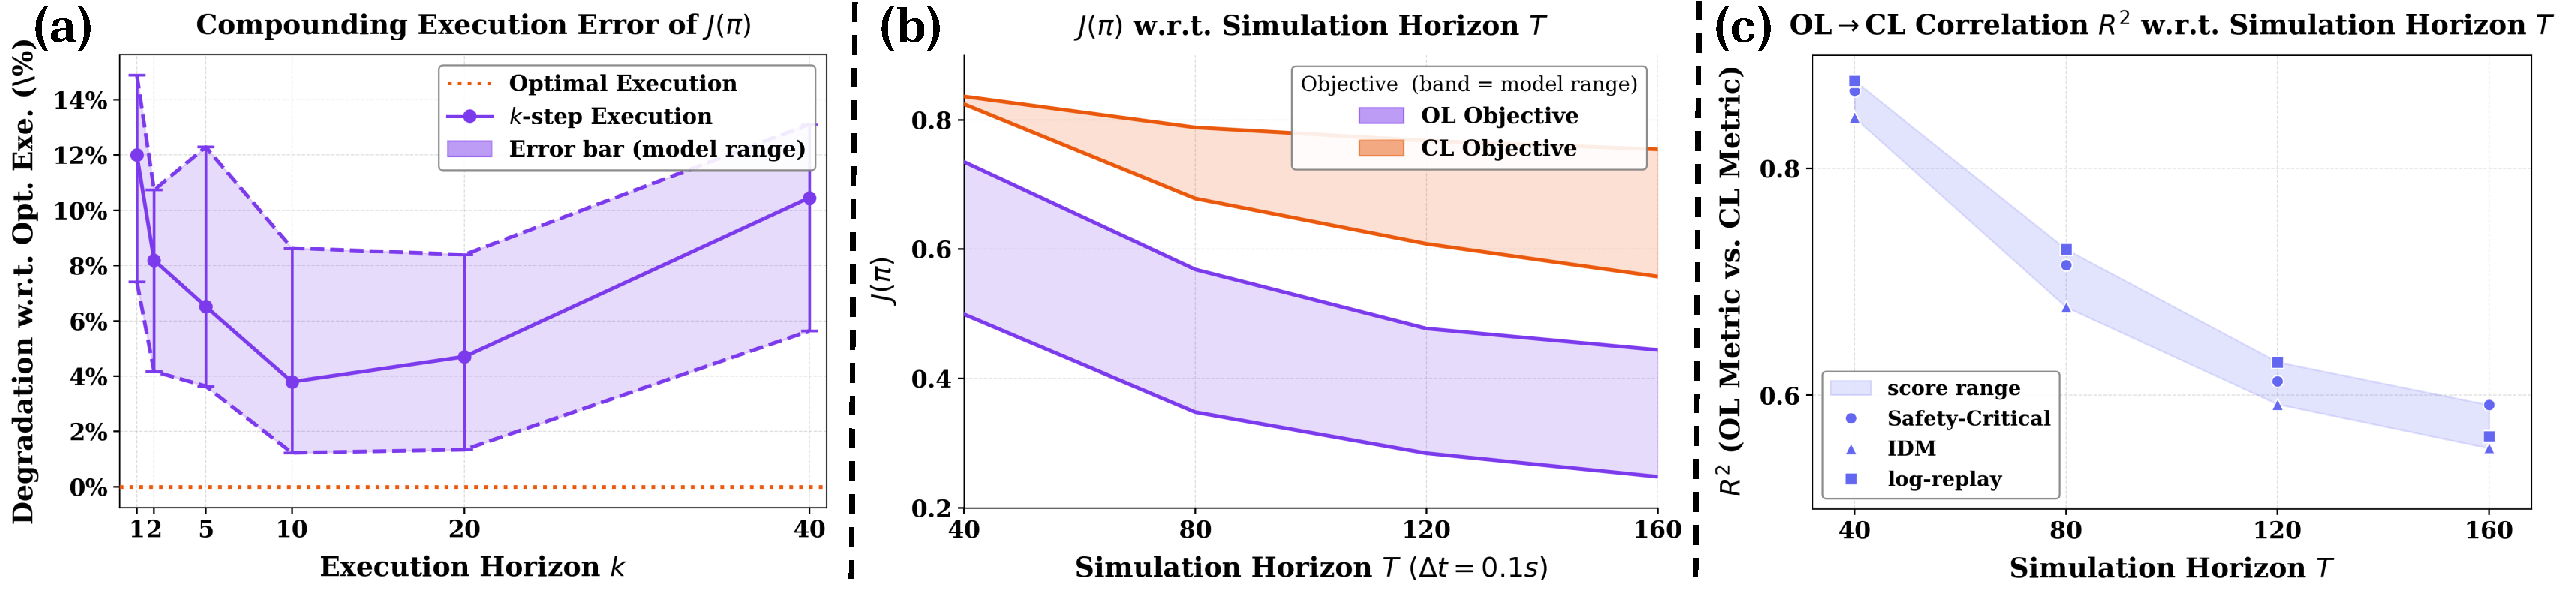
\includegraphics[width=0.99\linewidth]{figs/3.3_empirical_new.pdf}
    \vspace{-1em}
    \caption{\textbf{目标错配的实证研究。} \textbf{(a)}：$J(\pi)$ 随执行时域 $k$ 变化的累积执行误差；\textbf{(b)}：闭环与开环目标下的 $J(\pi)$，两条曲线之间的发散构成目标错配差距（$\Delta_{\mathrm{obj}}$）；\textbf{(c)}：不同交通模式下开环-闭环皮尔逊相关系数随仿真时域 $T$ 的变化。实验细节见附录~\ref{appendix:objective_mismatch_details}。}
    \label{fig:empirical_objective_mismatch}
    \vspace{-1em}
\end{figure}

有偏的Q值估计是开环训练的副产品，因为端到端规划器通常被优化为最小化整个预测序列 $H$ 上的误差。这在数学上等价于优化开环目标 $J_{\mathrm{OL}}(\pi) \approx J_H(\pi)$，其中执行时域 $k$ 被隐式强制等于规划时域 $H$。在 $J_H(\pi)$ 下，未来状态通过开环运动学假设展开，从根本上忽视了环境随机性、累积协变量偏移以及其他交通参与者的反应式行为。因此，这些离线代理分布与高频主动执行所诱导的真实闭环状态访问分布 $d^{\pi_{\theta, \phi}}$ 从根本上脱节。

与此并行的是，开环训练的静态特性无法灌输顺序决策所需的时间鲁棒性，使策略容易受到累积执行误差的影响。由于策略并未训练为在连续高频执行中保持稳定性，朴素的 $k$ 步执行策略很难获得最优闭环回报，如图~\ref{fig:empirical_objective_mismatch}(a) 所示。我们将这些因素导致的累积性能下降形式化为\emph{目标错配差距（Objective Mismatch Gap）}：
\begin{equation}
\small
    \Delta_{\mathrm{obj}}(\theta) \triangleq J_{k^*}(\pi_{\theta, \phi_{\mathrm{CL}}}) - J_{k=H}(\pi_{\theta, \phi_{\mathrm{OL}}}),
\end{equation}
其中 $\phi_{\mathrm{CL}}$ 表示在诱导分布 $d^{\pi_{\theta, \phi}}$ 上、通过最优执行 $k*$ 在统一闭环目标下优化的解码器参数；$\phi_{\mathrm{OL}}$ 则表示在离线专家状态分布下仅通过开环代理目标（$k=H$）优化的解码器。基于这一形式化，我们假设目标错配构成闭环迁移的主要结构性障碍。具体而言，我们预计依赖开环代理目标会导致优化目标发散，从而无法最大化闭环回报。

\textbf{实证研究。}为检验这一假设，我们在代表性的端到端策略家族~\cite{diffusiondrive, diffusiondrivev2, transfuser, RAP} 上实证刻画目标错配（$\Delta_{\mathrm{obj}}$）随仿真时域 $T$ 的变化，如图~\ref{fig:empirical_objective_mismatch}(b) 所示。我们跟踪开环与闭环目标下回报的发散程度。关键在于，当 $T$ 恰好超过 $H$ 时，性能差距显著扩大。这一趋势证实了我们的假设，表明有偏的Q值估计不足以评估长时域交互中的状态-动作值。此外，图~\ref{fig:empirical_objective_mismatch}(c) 显示，当 $T > H$ 时，开环与闭环指标之间的皮尔逊相关系数急剧衰减，证明标准开环评估可能对闭环部署就绪程度得出误导性结论。我们的分析表明：\textbf{OL-CL差距的主要根源在于目标错配，需要通过测试时自适应来显式纠正有偏的Q值估计和闭环执行中的顺序决策。}

%===============================================================================

\section{提出的方法：测试时自适应（TTA）框架}
\label{section:method}

受第~\ref{section:decomposition_analysis}~节分解分析的启发，我们提出测试时自适应（TTA）框架，在不进行额外端到端重训练的情况下提升开环预训练 $\text{E2E}$ 策略的闭环鲁棒性。该框架由两部分组成：通过流匹配恢复潜在表征的观测校准器（第~\ref{subsec:observational_calibrator}~节），以及缓解有偏的Q值估计、自适应执行以最大化最终闭环回报的策略自适应过程（第~\ref{subsec:test_time_adaptation}~节）。

\subsection{观测校准器}
\label{subsec:observational_calibrator}

如第~\ref{subsec:observational_shift}~节所述，我们在固定视觉编码器下、由观测通道诱导的潜在表征层面上形式化观测偏移。设 $f_\theta:\mathcal{O}\to\mathcal{Z}$ 为预训练编码器，$\Omega^{\mathrm{source}}(\cdot\mid s)$ 和 $\Omega^{\mathrm{target}}(\cdot\mid s)$ 分别表示源域和目标域中的观测通道。对于每个域 $d\in\{\mathrm{source},\mathrm{target}\}$，给定特定域的状态分布 $\rho^{d}$，我们将诱导的表征分布 $\mathcal{D}_{d}$ 定义为生成过程 $s\sim\rho^{d}$、$o\sim\Omega^{d}(\cdot\mid s)$ 下 $z=f_\theta(o)$ 的边缘分布。注意 $\mathcal{D}_{\mathrm{source}}$ 和 $\mathcal{D}_{\mathrm{target}}$ 都定义在 $\mathcal{Z}$ 上，但由于感知模型依赖域，两者通常不同。

随后，我们使用流匹配学习一个在前推意义下对齐这些分布的传输映射 $g:\mathcal{Z}\to\mathcal{Z}$，即 $g_{\#}\mathcal{D}_{\mathrm{source}}\approx \mathcal{D}_{\mathrm{target}}$ \cite{lipman2022flow}，从而使从源域观测提取的潜在特征能够被映射为与下游策略 $\pi_\phi$ 兼容的表征。为提高对齐性能，我们并不单纯依赖朴素的流匹配目标，而是受 \cite{liu2025flowing} 启发，用多目标损失优化校准器。我们在图~\ref{fig:empirical_observational_shift} 中通过潜在特征对齐以及开环、闭环指标的相应恢复，表明这种校准能有效缓解观测域偏移。多目标损失的精确公式以及数据集构建和模型架构的更多实现细节见附录~\ref{appendix:observational_calibrator}。

\begin{figure}[tbh]
    \centering
    
\includegraphics[width=0.99\linewidth]{figs/4.2.pdf}
    \vspace{-1em}
    \caption{\textbf{测试时策略自适应。} \textbf{(a)}：截断Q值估计器在闭环执行期间选择安全的规划轨迹；\textbf{(b)}：若新提出的轨迹未获得更高的Q值，自适应重规划保留先前已验证的规划轨迹；\textbf{(c)}：有偏（基线）与截断Q值估计器（TTA）之间的测试时扩展动力学。}
    \label{fig:test_time_policy_adaptation}
    \vspace{-1em}
\end{figure}

\subsection{测试时策略自适应}
\label{subsec:test_time_adaptation}

\subsubsection{截断Q值估计}
\label{subsubsec:intrinsic_q_estimation}

% To mitigate the biased Q-value estimation learned from the open-loop proxy objective, we propose a truncated action-value estimator applied dynamically at test time.
为消除通过开环代理目标学到的Q值估计器固有的偏差，我们提出一种动态的、测试时的截断动作值估计器。
在任意决策步 $t$，随机策略 $\pi^{\Omega}_{\theta, \phi}(\cdot \mid s_t)$ 输出 $N$ 个候选轨迹-动作的离散集合，记为 $\mathcal{A} = \{\mathbf{a}^{(1)}, \dots, \mathbf{a}^{(N)}\}$。每个候选 $\mathbf{a}^{(i)}$ 表示一个由覆盖整个规划时域 $H$ 的原始控制组成的独特时空规划。

评估所选前缀轨迹的质量通常依赖于 $k$ 步执行前缀上的即时奖励之和与期望未来回报 $\gamma^k \mathbb{E} [ V^\pi(s_{t+k}) ]$。然而，这种标准期望回报隐式地将奖励无限累积到未来。依赖开环转移模型估计远超显式规划时域 $H$ 的状态，本质上会引入累积协变量偏移和未建模的环境随机性，使无偏估计在实践中难以实现。

为克服这一问题，我们引入截断动作值估计器，将估计严格限制在可靠的规划时域 $H$ 内：
\begin{equation}
\small
    \label{eq:q_estimator_exact}
    \hat{Q}^{\pi}(s_t, \mathbf{a}_t) \triangleq R_k(s_t, \mathbf{a}_t) + \gamma^k \mathbb{E} \left[ V^\pi(s_{t+k}) \right] - \gamma^H \mathbb{E} \left[ V^\pi(s_{t+H}) \right],
\end{equation}
其中 $\gamma \in [0, 1)$ 是折扣因子，$R_k(s_t, \mathbf{a}_t) = \sum_{i=0}^{k-1} \gamma^{i} r(s_{t+i}, \mathbf{a}_{t+i})$ 严格捕获执行前缀 $k$ 上的即时几何与历史惩罚。

通过显式减去终端时域极限处的折扣期望值 $\gamma^H \mathbb{E} [ V^\pi(s_{t+H}) ]$，我们从数学上消去了难以处理的无穷尾项。这确保 $H$ 之外的值估计被安全忽略，将估计器限制在模型显式时空规划所界定的高置信窗口内进行评估。期望Q函数的实现详见附录~\ref{appendix:test-time-adaptation}。

如图~\ref{fig:test_time_policy_adaptation}(a) 所示，在闭环执行过程中，智能体不再默认采用有偏开环策略~\cite{diffusiondrivev2, diffusiondrive} 中得分最高的序列，而是选择最大化 $\hat{Q}^{\pi}$ 的候选轨迹。该机制在每个决策步持续运行，动态过滤掉遭受第~\ref{subsec:objective_mismatch}~节所述有偏估计影响的规划。

\subsubsection{自适应重规划}
\label{subsubsec:adaptive_replan}

标准测试时评分器通常以无记忆方式运行，仅从策略提出的当前候选集 $\mathcal{A}_t$ 中选择，这常常导致高频动作抖动和连续规划周期之间的时间不一致。为克服累积执行误差，我们保留先前已验证规划中未执行的路径点，并提出自适应重规划机制，在需要时自适应地执行重规划，如图~\ref{fig:test_time_policy_adaptation}(b) 所示。

设 $\mathbf{a}^*_{\mathrm{prev}}$ 为上一规划周期（步 $t-k$）选择的最优轨迹。在当前决策步 $t$，智能体已完成 $k$ 步执行前缀。为严谨评估是否保留现有规划，我们提取其包含 $H-k$ 个路径点的未执行部分，并将其空间变换到 $s_t$ 处的自车中心坐标系。我们将这一变换后的持久规划记为 $\mathbf{a}_{\mathrm{rem}}$。为确保与新生成候选 $\mathbf{a} \in \mathcal{A}_t$ 的公平比较，我们用公式~\ref{eq:q_estimator_exact} 中 $\hat{Q}^{\pi}$ 在缩短时域上的积分来估计期望回报，将 $\mathbf{a}_{\mathrm{rem}}$ 的截断动作值分别与每个新候选对应的 $(H-k)$ 步前缀（记为 $\mathbf{a}_{[:H-k]}$）进行比较。

如果持久规划的估计 $Q$ 值等于或超过任一新候选对应前缀的值，则保留该持久规划：
\begin{equation}
\small
    \mathbf{a}_t^* =
    \begin{cases}
        \mathbf{a}_{\mathrm{rem}} & \text{if } \hat{Q}^{\pi}(s_t, \mathbf{a}_{\mathrm{rem}}) \ge \max\limits_{\mathbf{a} \in \mathcal{A}_t} \hat{Q}^{\pi}(s_t, \mathbf{a}_{[:H-k]}), \\
        \arg\max\limits_{\mathbf{a} \in \mathcal{A}_t} \hat{Q}^{\pi}(s_t, \mathbf{a}) & \text{otherwise}.
    \end{cases}
\end{equation}
仅当新生成的候选在共享时间时域上产生严格更优的期望回报时，智能体才会放弃持久规划。

\section{实验}
\label{section:experiments}

\subsection{实验设置}
我们以BridgeSim平台作为仿真引擎和基准，场景与交通模式可通过场景描述加载，详见附录~\ref{appendix:bridgesim_platform}。基线方法包括在NAVSIM~\cite{navsimv2} 上预训练的 DiffusionDrive~\cite{diffusiondrive}、DiffuionDriveV2~\cite{diffusiondrivev2} 和 RAP~\cite{RAP}。我们在以下三种设置下评估所提出的TTA框架：1) \textbf{域内评估}：模型在不同的仿真时域下于NavHard测试集的日志回放场景中测试；2) \textbf{未见场景评估}：模型在与预训练域不同的日志回放场景中测试，如 nuScenes~\cite{caesar2020nuscenes}、WOMD~\cite{mei2022waymo}；3) \textbf{反应式评估}：模型在NavHard场景中测试，其中交通智能体被替换为IDM~\cite{idm} 或对抗模式~\cite{advbmt}。闭环指标包括一个 \textit{BridgeSim 驾驶得分}（Driving Score, \textbf{DS}），它是扩展预测驾驶员模型得分（Extended Predictive Driver Model Score, \textbf{EPDMS}）与路线完成率（Route Completion, \textbf{RC}）的复合得分。注意，\textbf{EPDMS} 是基于无过错碰撞（No At-Fault Collisions, \textbf{NC}）、可行驶区域合规（Drivable Area Compliance, \textbf{DAC}）、信号灯合规（Traffic Light Compliance, \textbf{TLC}）、行驶方向合规（Driving Direction Compliance, \textbf{DDC}）、车道保持（Lane Keeping, \textbf{LK}）、碰撞时间（Time-to-Collision, \textbf{TTC}）、历史舒适度（History Comfort, \textbf{HC}）和扩展舒适度（Extended Comfort, \textbf{EC}）的复合指标。指标细节见附录~\ref{appendix:eval_metrics}，更多实验细节见附录~\ref{appendix:cl_eval_details}。

\subsection{主要结果}
\textbf{域内评估结果。}如图~\ref{fig:main_exp}(a) 所示，我们在BridgeSim-NavHard场景中，以 4/8/12/16 秒的不同仿真时域评估日志回放场景。由于累积协变量偏移，端到端规划器的可靠性通常随仿真时域的增加而下降。TTA的引入显著平缓了所有基线智能体上的这条衰减曲线。通过执行与闭环对齐的测试时自适应，该框架缓解了\textit{目标错配}问题。结果表明，TTA使智能体能够在长时域闭环仿真中保持更高的时间一致性和安全得分。

\begin{figure}[tbh]
    \centering
    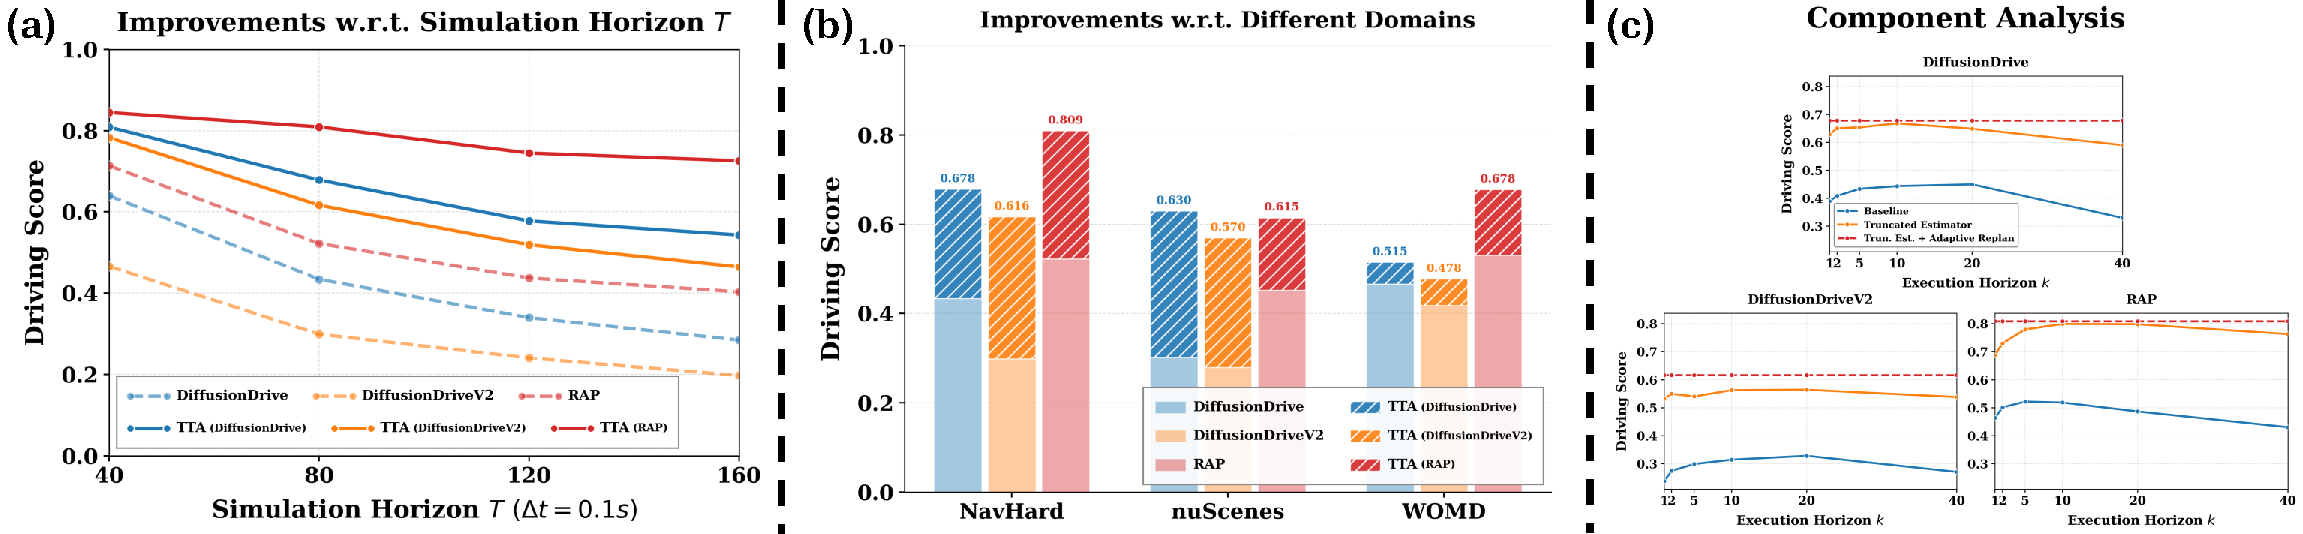
\includegraphics[width=0.99\linewidth]{figs/5.1_main.pdf}
    \vspace{-1em}
    \caption{\textbf{所提出TTA框架的改进效果。} (a)：BridgeSim-NavHard场景中不同仿真时域下的性能增益；(b)：不同日志回放域下的性能增益；(c)：TTA框架的组件分析。}
    \label{fig:main_exp}
    \vspace{-1em}
\end{figure}

\textbf{未见场景评估结果。}如图~\ref{fig:main_exp}(b) 所示，所提出的TTA框架在与多种开环基线~\cite{diffusiondrive, diffusiondrivev2,RAP} 集成时产生一致的性能增益。这些改进在三个不同的评估环境中持续存在，即 NavHard~\cite{navsimv2}、nuScenes~\cite{caesar2020nuscenes} 和 WOMD~\cite{mei2022waymo}，证明了该框架的跨域鲁棒性。

\textbf{反应式评估结果。}如表~\ref{tab:reactive_cl_scores} 所示，我们评估了所提出的TTA框架在不同交通模式下提供的性能增益。结果表明，TTA在所有基线架构上持续改善关键闭环指标，如进度相关指标（\textbf{RC}）和安全相关指标（\textbf{TTC} 和 \textbf{NC}）。这些结果证明了TTA框架在反应式仿真中以稳健的安全约束实现效率的有效性。

\textbf{组件分析。}如图~\ref{fig:main_exp}(c) 所示，我们解耦TTA各模块的贡献，以评估它们对最终性能的单独影响。结果表明，所提出的截断Q值估计器在所有测试的执行时域 $k$ 上都显著优于原始的有偏基线。此外，自适应重规划机制的加入持续识别最优的展开（rollout）轨迹，有效缓解累积执行误差，从而在不同主干网络上获得更稳健、更稳定的驾驶得分。

\begin{table}[tbh]
\centering
\caption{不同反应式交通模式下的性能对比。注意，TTA改善了\textbf{NC}、\textbf{TTC}和\textbf{RC}等关键闭环指标，从而总体上获得更高的\textbf{DS}。完整的子指标得分见附录~\ref{appendix:detailed_reactive_metrics}。}
\label{tab:reactive_cl_scores}
\renewcommand{\arraystretch}{1.5}
\setlength{\aboverulesep}{0pt}
\setlength{\belowrulesep}{0pt}
\resizebox{\textwidth}{!}{
\begin{tabular}{l *{7}{c} @{\hspace{6pt} } *{7}{c}}
\toprule
\multirow{2}{*}{\textbf{模型}} & \multicolumn{7}{c}{\textbf{IDM}} & \multicolumn{7}{c}{\textbf{安全关键}} \\
\cmidrule(lr){2-8} \cmidrule(lr){9-15}
 & \textbf{DS} & \textbf{EPDMS} & \textbf{RC} & \textbf{NC} & \textbf{DAC} & \textbf{TTC} & \textbf{LK} & \textbf{DS} & \textbf{EPDMS} & \textbf{RC} & \textbf{NC} & \textbf{DAC} & \textbf{TTC} & \textbf{LK} \\
\midrule
DiffusionDrive & 45.30 & 72.95 & 59.93 & 95.41 & 85.47 & 89.73 & 89.83 & 38.68 & 68.16 & 54.77 & 93.62 & 83.86 & 84.97 & 90.71 \\
DiffusionDriveV2 & 31.94 & 65.43 & 45.85 & 94.57 & 82.09 & 89.10 & 85.42 & 28.17 & 61.45 & 43.50 & 93.15 & 80.78 & 85.72 & 85.81 \\
RAP & 60.02 & 76.85 & 77.20 & 97.68 & 88.84 & 93.07 & 78.16 & 51.83 & 70.88 & 71.22 & 95.03 & 88.16 & 86.37 & 78.26 \\
\midrule
\rowcolor{green!15} TTA \scriptsize (DiffusionDrive) & 62.68 \scriptsize \textcolor{red}{+17.4} & 84.36 & 72.28 & 96.85 & 95.63 & 91.57 & \textbf{92.43} & 55.02 \scriptsize \textcolor{red}{+16.3} & 78.95 & 67.92 & 94.73 & 95.21 & 86.64 & \textbf{91.30} \\
\rowcolor{green!15} TTA \scriptsize (DiffusionDriveV2) & 53.96 \scriptsize \textcolor{red}{+22.0} & 77.47 & 67.89 & 96.08 & 90.53 & 89.46 & 89.98 & 47.64 \scriptsize \textcolor{red}{+19.5} & 71.66 & 65.91 & 93.54 & 89.16 & 84.23 & 90.11 \\
\rowcolor{green!15} TTA \scriptsize (RAP) & \textbf{79.07} \scriptsize \textcolor{red}{+19.1} & \textbf{90.92} & \textbf{86.21} & \textbf{98.28} & \textbf{98.62} & \textbf{95.31} & 91.52 & \textbf{65.94} \scriptsize \textcolor{red}{+14.1} & \textbf{82.01} & \textbf{78.66} & \textbf{95.30} & \textbf{96.19} & \textbf{87.71} & 90.26 \\
\bottomrule
\end{tabular}
}
\vspace{-1em}
\end{table}

\textbf{测试时扩展动力学。}我们沿用~\cite{diffusiondrive, diffusiondrivev2, li2025ztrs, yao2026drivesuprim}，在开环指标上展示轨迹提议测试时扩展的收益。如图~\ref{fig:test_time_policy_adaptation}(c) 所示，闭环仿真中不同评分机制的对比实验表明，测试时扩展动力学高度依赖于评分器的质量。我们提出的评分器持续受益于更广状态访问下的扩展，而有偏的Q值估计器则无法达到类似的改进。

\section{结论}
本文对端到端自动驾驶中的OL-CL差距进行了深入分析，表明开环优化并不能保证长时域闭环仿真中的安全或稳定行为。因此，我们的分析揭示，仅仅扩展开环训练不足以实现现实部署。相反，需要对观测模块和策略模块都应用针对性的测试时自适应（如我们提出的TTA框架），才能在闭环部署中获得安全稳健的驾驶行为。我们的发现还表明，端到端驾驶在开环基准上已接近饱和。在这一平台期，开环指标对现实世界闭环能力的预测可靠性仍然存疑。未来方向方面，我们认为端到端驾驶研究应将重心转向更现实的闭环评估和目标对齐学习，在闭环设置中直接改进驾驶模型。

% \section{Limitations}
% To add during the CoRL submission
% 1. Doesn't talk about closed-loop training
% 2. Closed-loop simulation is costly

\clearpage
% The acknowledgments are automatically included only in the final and preprint versions of the paper.
% \acknowledgments{If a paper is accepted, the final camera-ready version will (and probably should) include acknowledgments. All acknowledgments go at the end of the paper, including thanks to reviewers who gave useful comments, to colleagues who contributed to the ideas, and to funding agencies and corporate sponsors that provided financial support.}

%===============================================================================

% no \bibliographystyle is required, since the corl style is automatically used.
\bibliography{example}  % .bib
\newpage
\appendix

\section*{附录}
\section{更多相关工作}
\label{appendix:more_related_works}
\textbf{端到端驾驶策略自适应。}端到端（E2E）驾驶策略的自适应长期在模仿学习的协变量偏移这一更广泛问题下被研究。当策略遇到分布外状态时，行为克隆会遭受累积误差，这推动了 DAgger 等交互式学习方法的发展，这些方法通过策略内数据聚合解决行为分布偏移~\cite{ross2011dagger, ross2014reinforcement}。在驾驶特定设置中，先前研究证实，大规模开环模仿学习常常过拟合静态专家轨迹，并在长时域或反应式交互下失效~\cite{codevilla2019exploring,zheng2024datascalinglaw}。
与行为偏移正交，仿真到现实（sim-to-real）迁移研究强调观测分布偏移是端到端策略的关键失效模式~\cite{dosovitskiy2017carla}。虽然域随机化和表征学习可以提高鲁棒性，但它们并不能显式保证异构仿真器之间的规划导向保真度。近期的开环基准支持可扩展的评估，但已被证明与闭环可靠性相关性较弱，凸显了静态评估协议的局限~\cite{navsimv1, navsimv2}。与先前单独处理感知或策略偏移的工作不同，我们的工作对OL–CL差距进行了深入分解，并在受控的、仿真器诱导的转移变化下研究二者的交互。

\section{BridgeSim平台更多细节}
\label{appendix:bridgesim_platform}

\subsection{动机}
BridgeSim平台是一个统一的跨仿真器闭环仿真平台，支持端到端策略在不同仿真器上进行评估，如图~\ref{fig:bridgesim_platform} 所示。我们认为，现有基准测试平台不足以对端到端自动驾驶中的OL-CL差距进行严谨而统一的分析。现有端到端驾驶基准的局限可归结为三个主要缺陷：1) 现有基准~\cite{navsimv1, navsimv2} 中的开环评估通常只与短期闭环性能存在表面相关性，无法作为长时域闭环能力的可靠指标；2) 当前闭环基准常常缺乏多视图时间一致性~\cite{yang2024drivearena}，对观测一致的交通元素标注不准确~\cite{zhou2024hugsim}，或缺乏压力测试泛化能力所需的环境多样性和智能体行为~\cite{jia2024bench}（更多细节见附录~\ref{appendix:current_e2e_bottlenecks}）；3) 在仿真器之间迁移的策略常常遇到不一致的车辆动力学和控制器配置，导致人为的性能下降，掩盖了真实的OL-CL差距。

这些系统性缺陷决定了BridgeSim平台的设计：该平台被设计为可控的，以便识别模块化变化，并在评估模式和指标上保持一致。为此，BridgeSim利用 MetaDrive~\cite{li2022metadrive, li2023scenarionet} 仿真引擎来解决以往基准中普遍存在的可控性和不一致性问题。如图~\ref{fig:bridgesim_platform} 所示，BridgeSim通过模块化架构确保高保真闭环仿真，实现了：1) 统一的策略迁移结构框架，以保持跨域的状态-动作兼容性；2) 统一的场景协议，实现精确、可重复的环境回放和可控的智能体交互；3) 统一的评估模式与指标，确保公平准确的比较。

\begin{figure}[tbh]
    \centering
    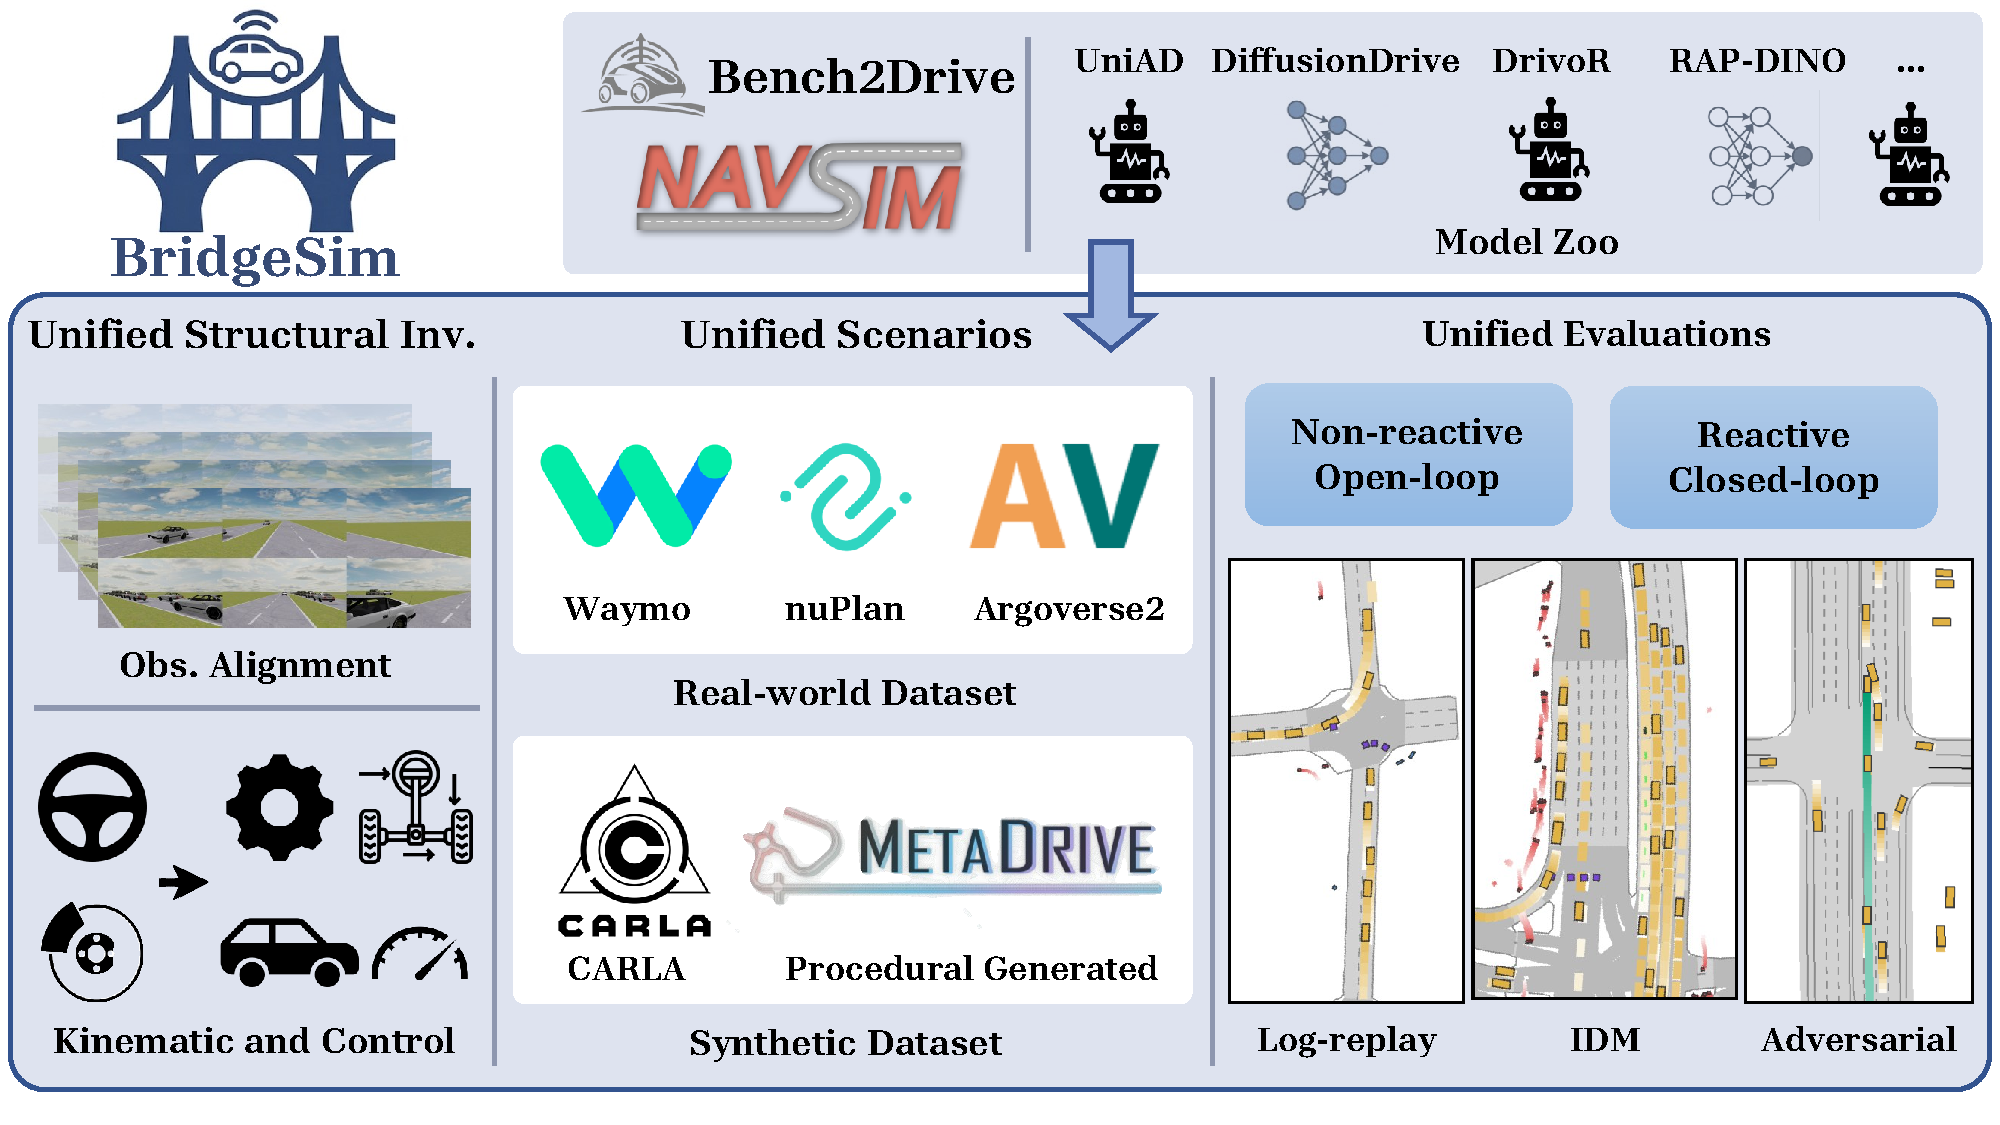
\includegraphics[width=0.99\linewidth]{figs/bridgesim.pdf}
    \vspace{-1em}
    \caption{BridgeSim平台示意图。BridgeSim支持对来自任何其他仿真器的预训练策略进行统一的闭环仿真，使我们能够进行严谨的分解分析。}
    \label{fig:bridgesim_platform}
\end{figure}

\subsection{策略迁移中的统一结构不变性}
为量化 $\text{OL-CL}$ 差距，必须将策略的决策逻辑与混杂的系统变量解耦。为建立公平的诊断框架，BridgeSim在两层上强制结构不变性：

\textit{1) 观测对齐：}我们在所有评估的基准上标准化传感器配置，包括相机外参和内参。这种标准化确保性能失败严格归因于策略的表征鲁棒性，而非输入空间 $\Omega$ 中表面的几何错配。由于仿真器保持严格的物理特性，我们进一步强制多视图时间一致性，以解决现有基准中的常见缺陷。传感器观测 $o_t$ 通过几何投影合成，确保 $o_t$ 在所有相机帧和时间步上与底层状态 $s_t$ 保持空间和时间一致性。这种方法消除了虚假的分布偏移，从而确保策略失败根源于决策错误而非仿真伪影。现有生成式和基于高斯泼溅的仿真范式的代表性失败案例详见附录~\ref{appendix:current_e2e_bottlenecks}。

\textit{2) 运动学与控制对齐：}我们在车辆动力学和控制执行层上强制一致性，以隔离性能下降的来源。通过在预测路径点的执行过程中标准化转移动力学 $\mathcal{P}$，我们确保所测得的 $\text{OL-CL}$ 差距反映的是根本的规划层面失败，而非下游执行差异。为确保我们的评估反映标准实践，我们采用各类真实世界自动驾驶平台中普遍使用的控制器~\cite{christensen2021autonomous}：具体而言，纵向控制采用标准PID公式，横向跟踪采用纯追踪（Pure Pursuit）~\cite{coulter1992implementation} 控制器。此外，BridgeSim通过将这些车辆动力学与渲染流程显式解耦，保持严格的结构不变性。

\subsection{统一场景协议}
\textbf{场景描述。}我们定义了一个统一的、序列化的数据模式，用于封装重建任意驾驶回合所需的全部静态和动态元素。为确保跨平台兼容性，转换器将来自真实世界日志（如 Waymo~\cite{mei2022waymo}、nuScenes~\cite{caesar2020nuscenes}）和合成环境（如 CARLA~\cite{jia2024bench}）的多样源数据映射为标准的 \texttt{ScenarioDescription} 格式。

这一集中的数据结构包含三个主要部分：

\textit{1) 地图特征。}BridgeSim通过标准化协议摄取包括 Waymo~\cite{mei2022waymo}、nuPlan~\cite{caesar2021nuplan}、nuScenes~\cite{caesar2020nuscenes} 在内的多样真实世界数据集，以提取地图几何。该几何被离散化并存储为密集点序列，每个点被赋予特定的类型属性。随后，我们将高精地图（HD Map）元素（如车道、边界、人行横道和停止线）矢量化到统一的多段线表征中。通过在仿真环境中确保这些布局的精确空间对齐，我们消除了可能扭曲车道属性的渲染伪影，从而比现有基准保持更高的保真度和一致性。

\textit{2) 目标轨迹。}动态智能体以时间轨迹存储，包含状态序列，包括 $position$、$heading$、$velocity$、$dimensions$ 以及有效性掩码。为解决不同数据集采样率不同的问题，我们实现了对轨迹进行上采样的插值流程。该过程对位置和速度使用线性插值，对航向应用角度插值，以确保仿真期间平滑的运动学回放。

\textit{3) 动态地图状态。}信号灯状态与静态地图几何解耦。我们将单个交通信号映射到特定车道ID，并存储其状态序列（如 \textit{STOP}、\textit{WAIT}、\textit{GO}）。这种映射使仿真器能够在回放期间动态更新车道信号，确保智能体的行为约束与视觉环境保持同步。

\textbf{交通模式。}BridgeSim提供用于动态配置智能体行为的API，以便在不同交互水平下对策略进行压力测试。我们支持以下智能体行为模式：

\textit{1) 日志回放模式。}在该模式下，背景智能体严格遵循源数据集中记录的轨迹。仿真器本质上回放预设的车辆轨迹。虽然这保留了真实世界的精确上下文，但这些智能体对自车的偏离不作反应。

\textit{2) IDM模式}~\cite{idm}。为弥合静态数据集与闭环交互之间的差距，我们用智能驾驶员模型（IDM）替代日志回放策略。背景车辆以其真值位姿初始化，其后续行为由启发式策略支配。这些智能体遵循车道几何、保持安全间距，并主动响应自车的存在。

\textit{3) 对抗模式。}我们提供将对抗性智能体~\cite{advbmt} 注入日志回放场景的接口。这使得能够生成安全关键的边缘案例，促使自车策略即时反应以避免迫近的碰撞。

\textbf{坐标系。}跨不同仿真器评估策略的一个关键挑战是坐标系（如全局与局部、左手系与右手系）的不对齐。BridgeSim强制执行以局部场景锚点为中心的统一右手坐标系（RHS）。我们采用以下技术确保坐标系对齐：

\textit{1) 手性归一化。}对于使用左手坐标系的数据集（如 CARLA、Bench2Drive），我们在转换期间应用基变换。方向角（偏航角、横滚角）相应取反，以保持运动学一致性。

\textit{2) 空间锚定。}为减轻大规模全局坐标（在 nuScenes 和 nuPlan 中常见）固有的浮点误差，我们将所有空间数据相对于场景锚点进行归一化，锚点定义为 $t=0$ 时自车的位置。所有地图特征和轨迹都被平移，使地图原点与该锚点对齐，为规划器和仿真器物理引擎确保数值稳定性。

\textbf{时间长度。}BridgeSim支持由源日志完整范围决定的长期仿真时长，从而将仿真时域与源仿真器解耦。场景时长也可以手动配置为可变长度，即完整源场景的子时长。为适应这些多样数据集异构的采样率，我们实现了标准化的轨迹插值协议。该流程使用线性和角度插值将源信号重采样到仿真器原生的10Hz控制频率。这确保了不同时间步上一致的运动学评估，且不会人为截断场景。

\subsection{统一评估模式与指标}
\label{appendix:eval_metrics}
\textbf{评估模式。}为严谨评估驾驶智能体从离线数据集泛化到在线部署的能力，BridgeSim实现了统一的评估流程。该流程在同一环境 $\mathcal{E}$ 内同时支持\textit{非反应式开环评估}和\textit{反应式闭环评估}。设 $\mathcal{S}$ 为状态空间，$\mathcal{A}$ 为动作空间。在时间 $t$，智能体观测状态 $s_t \in \mathcal{S}$ 并生成规划轨迹 $\tau_t = \pi(s_t)$。

\textit{1) 非反应式开环仿真。 }在开环模式下，仿真将自车的轨迹规划与环境的状态转移解耦。环境动力学严格由源数据集的真值轨迹支配。在该模式下，自车的状态转移被强制匹配日志中的轨迹 $\mathcal{T}_{log}$，与策略输出无关。具体而言，状态转移定义为 $s_{t+1} = f(s_t, a^*_{t})$，其中 $a^*_t$ 表示日志中记录的专家动作。模型在每个时间步预测轨迹 $\hat{\tau}_t$，并将其从自车坐标系变换到全局仿真坐标系，以对照静态地图和动态智能体（从日志回放）进行评估。该模式隔离了规划器的推理能力，不涉及累积控制误差这一混杂因素。

\textit{2) 反应式闭环仿真。 }在闭环模式下，评估关注智能体在长时域内稳健控制车辆的能力。仿真环境可配置为\textit{全反应式}范式——背景交通行为由动态响应自车动作的智能驾驶员模型（IDM）支配——或\textit{半反应式}范式——背景交通严格遵循原始日志轨迹，而自车仍由策略进行物理控制。

\textbf{评估指标。}为量化BridgeSim环境中的驾驶性能，我们按照先前协议~\cite{navsimv1, navsimv2, zhou2024hugsim, yang2024drivearena, li2025hydra-mdp++} 实现了一组开环和闭环指标。对于非反应式开环仿真，我们采用EPDMS框架~\cite{navsimv1, navsimv2, li2025hydra-mdp++}。对于反应式闭环仿真，我们采用受 HUGSIM~\cite{zhou2024hugsim} 和 DriveArena~\cite{yang2024drivearena} 驾驶得分启发的复合指标。

\textit{1) 开环指标：扩展预测驾驶员模型得分}（\textbf{EPDMS}）。\textbf{EPDMS} 得分实现为安全关键约束与驾驶质量特征的加权组合，如表~\ref{tab:epdms_metrics} 所示。与L2位移误差不同，\textbf{EPDMS} 会惩罚物理上不可行或不安全的规划，即使它们模仿了日志。在每个帧上，我们将模型预测的轨迹变换到仿真坐标系，并对照静态和动态地图特征进行评分。给定帧的最终得分 $S_{EPDMS} \in [0, 1]$ 定义为关键布尔约束 $\mathcal{C}$ 的乘积与软指标 $\mathcal{F}$ 的加权和之积：
\begin{equation}
    S_{EPDMS} = \left( \prod_{c \in \mathcal{C}} \mathbb{I}_c \right) \cdot \left( \frac{\sum_{f \in \mathcal{F}} w_f \cdot v_f}{\sum_{f \in \mathcal{F}} w_f} \right),
\end{equation}
其中 $\mathbb{I}_c \in \{0, 1\}$ 是约束合规的指示函数，$v_f \in [0, 1]$ 是归一化的特征得分，$w_f$ 是相应的权重。

\begin{table}[tbh]
\centering
\caption{\textbf{EPDMS}各子得分的描述。}
\label{tab:epdms_metrics}
\small
\renewcommand{\arraystretch}{1.0} % Adds breathing room between rows
\begin{tabularx}{\columnwidth}{@{} l >{\raggedright\arraybackslash}X @{}}
\toprule
\textbf{指标} & \textbf{描述} \\ \midrule
\multicolumn{2}{@{}l}{\textbf{\textit{关键约束（$\mathcal{C}$）}}} \\ \addlinespace
无过错碰撞（\textbf{NC}） & 自车多边形 $\mathcal{P}_{ego}$ 不得与任何回放目标的多边形 $\mathcal{P}_{obj}$ 相交。 \\
可行驶区域合规（\textbf{DAC}） & 整个时域必须满足高精地图内的 $\mathcal{P}_{ego} \subset \mathcal{M}_{drivable}$。 \\
信号灯合规（\textbf{TLC}） & 智能体不得越过与红灯状态相关的停止线。 \\
行驶方向合规（\textbf{DDC}） & 航向偏差 $|\theta_{ego} - \theta_{lane}|$ 必须保持在 $\pm \pi/2$ 以内。 \\ \midrule
\multicolumn{2}{@{}l}{\textbf{\textit{质量特征（$\mathcal{F}$）}}} \\ \addlinespace
自车进度（\textbf{EP}） & 将智能体进度表示为相对近似安全上界的比率。 \\
车道保持（\textbf{LK}） & 检查自车是否跟随当前车道的中心线，并避免在相邻车道间徘徊。 \\
碰撞时间（\textbf{TTC}） & 若投影的碰撞时间过低，则对轨迹 $\hat{\tau}$ 施加惩罚。 \\
历史舒适度（\textbf{HC}） & 用人类驾驶员的一小段历史运动评估规划器预测的轨迹。 \\
扩展舒适度（\textbf{EC}） & 限制运动学导数以保证乘客舒适：加速度 $a \le 4.89$，急动度 $j \le 8.37$，偏航率 $\dot{\theta} \le 0.95$。 \\
\bottomrule
\end{tabularx}
\end{table}

\textit{2) 闭环指标：BridgeSim驾驶得分。}对于反应式闭环仿真，我们将最终驾驶得分 $S_{CLS}$ 定义为智能体的全局路线完成率（\textbf{RC}）与帧级得分（$S_{EPDMS}^{(t)}$）时间平均值的乘积：
\begin{equation}
S_{CLS} = R_c \times \frac{1}{T} \sum_{t=1}^{T} S_{EPDMS}^{(t)},
\end{equation}

其中 $R_c\in[0, 1]$ 表示智能体相对于专家驾驶员路径或目标目的地完成的路线百分比，$T$ 是仿真回合中的总帧数，$S_{EPDMS}^{(t)}$ 是时间步 $t$ 的EPDM得分。注意，开环EPDMS评分中的帧级自车进度得分（\textbf{EP}）被移除，因为进度现在由仿真器中向目标行驶的距离显式度量~\cite{zhou2024hugsim}。关键在于，对于闭环设置，软特征集 $\mathcal{F}$ 被修改为排除位移误差或基于进度的项，仅关注驾驶质量和安全约束。该公式确保智能体只有在完成路线且在整个回合中始终保持安全舒适的驾驶行为时，才能获得高分。

\subsection{跨仿真器的仿真间评估结果}

\subsubsection{支持的模型库}
我们收录了一组多样化的公开端到端驾驶模型，用于零样本跨仿真器评估。除非另有说明，我们使用原作者或基准维护者发布的官方检查点。注意，按照附录~\ref{appendix:extensibility} 中的说明，新模型可以轻松集成到BridgeSim中。

\textbf{UniAD}~\cite{uniad} 是一个统一端到端自动驾驶框架，通过基于查询的Transformer架构联合建模感知、预测和规划。我们在评估中使用其官方Bench2Drive检查点。

\textbf{矢量化自动驾驶（Vectorised Autonomous Driving, VAD）}~\cite{vad} 是一种矢量化端到端驾驶方法，用结构化查询而非密集栅格特征表征地图元素和交通智能体。我们使用其官方Bench2Drive检查点。

\textbf{TransFuser}~\cite{transfuser} 是一种多模态端到端驾驶模型，融合RGB相机和LiDAR观测进行路径点预测。我们在评估中使用发布的NAVSIM训练检查点。

\textbf{DiffusionDrive}~\cite{diffusiondrive} 将自动驾驶形式化为使用锚定轨迹的截断扩散过程的生成式规划问题。我们评估中使用的发布检查点在NAVSIM上训练。

\textbf{DiffusionDriveV2}~\cite{diffusiondrivev2} 通过将强化学习（Reinforcement Learning, RL）纳入轨迹去噪过程来扩展DiffusionDrive。我们使用发布的NAVSIM训练检查点。

\textbf{LEAD}~\cite{LEAD} 研究模仿学习中的学习者-专家不对称性，并基于TransFuser-v6驾驶架构构建。发布的检查点包括用于 Leaderboard 2.0 / Bench2Drive 风格评估的基于CARLA的模型，以及LTFv6变体下的NAVSIM检查点。

\textbf{DrivoR}~\cite{DrivoR} 是一个基于Transformer的端到端规划器，构建在预训练的DINOv2视觉编码器之上，包含令牌压缩和轨迹评分模块。我们评估中使用的发布模型在NAVSIM上训练。

\textbf{栅格化增强规划（Rasterization Augmented Planning, RAP）}~\cite{RAP} 是一个基于栅格化的端到端驾驶增强框架，通过反事实栅格化视图和栅格到真实特征对齐改进训练。我们对比中使用的官方检查点在NAVSIM上训练。

\textbf{Alpamayo-R1}~\cite{wang2025alpamayo} 是一种用于端到端驾驶的视觉-语言-动作（Vision-Language-Action, VLA）模型，强调稳健的时间推理以处理复杂的城市机动。我们在评估中使用官方发布的检查点。

\textbf{OpenPilot}~\cite{openpilot2026} 是一个基于视觉的驾驶系统，利用多任务卷积神经网络预测路径、前车属性和车道边界。我们使用 comma.ai 提供的 v0.11.0 版本发布检查点。

\begin{table*}[h]
\centering
\caption{在BridgeSim-NavHard上评估的端到端驾驶策略的定量对比。所有结果均以重规划频率为 5、仿真时域为 8 秒报告。我们使用 $\mathrm{rr}=5$ 以与NAVSIM/OpenScene上训练常用的时间离散化对齐，该数据集以2\,Hz提供（即 $\Delta t = 0.5\,\mathrm{s}$）。}
\label{tab:appendix_main_results}
\resizebox{\textwidth}{!}{
\begin{tabular}{l|c|c|cc|cccccccc}
\toprule
\textbf{模型} & \textbf{预训练仿真器} & \textbf{DS} & \textbf{EPDMS} & \textbf{RC} & \textbf{NC} & \textbf{DAC} & \textbf{DDC} & \textbf{TLC} & \textbf{TTC} & \textbf{LK} & \textbf{HC} & \textbf{EC} \\
\midrule

人类专家 & N/A & 91.14 & 91.96 & 98.86 & 98.18 & 99.23 & 99.76 & 98.62 & 94.55 & 90.22 & 99.10 & 71.44 \\

\midrule

UniAD {\scriptsize (CVPR'23)} & Bench2Drive & 31.00 & 57.55 & 55.25 & 93.15 & 71.75 & 99.76 & 99.61 & 81.13 & 97.70 & 74.25 & 30.04 \\
VAD {\scriptsize (ICCV'23)} & Bench2Drive & 26.25 & 57.60 & 46.76 & 93.29 & 71.22 & 99.76 & 99.68 & 82.31 & 98.67 & 71.13 & 27.67 \\

\midrule

DiffusionDrive {\scriptsize (CVPR'25)} & NAVSIM & 43.29 & 69.70 & 61.30 & 95.38 & 81.48 & 99.76 & 98.81 & 87.47 & 91.57 & 91.64 & 39.02 \\
DiffusionDriveV2 {\scriptsize (arXiv)} & NAVSIM & 29.81 & 62.01 & 45.85 & 93.48 & 79.75 & 99.76 & 98.83 & 86.93 & 84.11 & 71.38 & 20.62 \\
RAP {\scriptsize (ICLR'26)} & NAVSIM & 52.08 & 72.41 & 70.74 & 95.63 & 85.24 & 99.76 & 99.18 & 88.14 & 84.69 & 92.84 & 48.91 \\
LEAD {\scriptsize (CVPR'26)} & NAVSIM & 26.34 & 54.02 & 47.42 & 93.29 & 68.44 & 99.53 & 99.89 & 84.70 & 96.38 & 91.62 & 36.59 \\
TransFuser {\scriptsize (PAMI'23)} & NAVSIM & 41.46 & 68.17 & 61.28 & 95.73 & 78.99 & 99.76 & 98.63 & 88.79 & 89.25 & 95.06 & 49.25 \\
LTF {\scriptsize (NeurIPS'24)} & NAVSIM & 50.10 & 69.29 & 70.64 & 95.49 & 78.80 & 99.53 & 98.51 & 88.61 & 90.28 & 95.02 & 58.27 \\
DrivoR {\scriptsize (CVPR'26)} & NAVSIM & 42.79 & 66.54 & 64.66 & 95.41 & 76.34 & 100.00 & 99.46 & 95.41 & 94.37 & 96.99 & \textbf{66.69} \\

\midrule

OpenPilot & Comma.ai & 64.75 & 79.50 & 82.21 & 97.55 & 94.29 & 100.00 & 98.89 & 92.58 & 84.43 & 92.12 & 62.06 \\
Alpamayo-R1 & Nvidia & 37.78 & 64.69 & 59.65 & 94.98 & 76.54 & 100.00 & 99.73 & 87.39 & 93.63 & 94.82 & 68.24 \\

\midrule
\rowcolor{green!15} TTA \scriptsize (DiffusionDrive) & NAVSIM & 67.84 & 79.77 & 82.54 & 96.48 & 87.03 & \textbf{100.00} & 99.01 & 96.07 & 91.85 & 36.18 & 33.72 \\
\rowcolor{green!15} TTA \scriptsize (DiffusionDriveV2) & NAVSIM & 61.46 & 76.86 & 77.86 & 95.83 & 86.80 & \textbf{100.00} & \textbf{99.17} & 92.93 & 91.51 & 26.22 & 24.32 \\
\rowcolor{green!15} TTA \scriptsize (RAP) & NAVSIM & \textbf{80.92} & \textbf{91.68} & \textbf{87.06} & \textbf{96.95} & \textbf{90.14} & \textbf{100.00} & 98.90 & \textbf{98.07} & \textbf{94.72} & 46.18 & 54.60 \\

\bottomrule
\end{tabular}}
\end{table*}

\subsubsection{仿真间评估结果}
我们在表~\ref{tab:appendix_main_results} 中的评估揭示，大多数开源模型在集成到BridgeSim平台时会遭受开环到闭环的部署差距。我们观察到，在合成仿真域上预训练的模型经常在视觉和行为两方面都遭遇仿真过拟合。具体而言，在Bench2Drive上训练的模型表现出显著的性能下降。这种差异凸显了CARLA的合成渲染与BridgeSim的真实世界回放场景之间存在显著的仿真间差距。另一方面，NAVSIM预训练模型表现更好，因为其训练环境依赖真实世界的交通行为。这些发现强调，除了视觉保真度外，行为真实感对于训练具有稳健仿真性能的自主智能体同样至关重要。结果表明，强大的域内性能并不总能转化为更广泛的泛化能力。

\subsection{支持新地图、新模型和新交通模式的可扩展设计}
\label{appendix:extensibility}

BridgeSim具有高度的向后兼容性和可扩展性，可以纳入新地图、新模型和新交通模式，鼓励开源贡献者在不修改任何共享评估逻辑的情况下，独立地用新颖的驾驶环境、最先进的规划模型和替代交通行为扩充该基准。

\textbf{纳入新地图。}要集成新地图，贡献者只需实现 \texttt{converter} 模块，并将新地图集成到场景描述协议中。该模块为每个支持的来源提供专门的、数据集特定的流程。每个流程实现一个转换函数，将原始的数据集原生记录转换为标准化的场景描述字典。通过在该函数内调用共享的序列化工具，生成的场景目录在评估期间可被环境管理器自动发现，无需修改下游评估逻辑。


\textbf{纳入新模型。}
贡献者可以使用 \texttt{adapter} 模块纳入新的规划器进行评估。我们通过抽象基类 \texttt{BaseModelAdapter} 提供接口，该接口包含四个核心函数以支持在BridgeSim上进行仿真：
\texttt{load\_model()} 用于检查点初始化和设备映射；
\texttt{prepare\_input()} 用于将原始多相机图像和自车状态向量转换为模型的原生输入格式；
\texttt{run\_inference()} 用于执行前向传播；
\texttt{parse\_output()} 用于提取自车坐标系中形状为
$N \times 2$ 的预测路径点轨迹。模型适配器实现后，只需在
\texttt{create\_model\_adapter()} 工厂中添加一个条目即可注册，之后新模型即可
立即在所有已加载的地图和交通模式下进行评估。

\textbf{纳入新交通模式。}
交通行为由 \texttt{EnvironmentManager} 组件支配，该组件将符号化的交通模式标识符映射到相应的MetaDrive仿真配置。要引入新的交通模式（如基于学习的交通生成模型或对抗性智能体策略），贡献者只需定义新的模式标识符，扩展内部配置解析器以输出必要的MetaDrive标志，并可选择提供自定义的智能体策略类。

\section{TTA框架实现细节}
\subsection{观测校准器实现细节}
\label{appendix:observational_calibrator}

观测校准器旨在通过流匹配框架对齐潜在表征分布 $\mathcal{D}_{\mathrm{source}}$ 和 $\mathcal{D}_{\mathrm{target}}$。为构建训练所需的特征对，我们利用NAVSIM数据集 \cite{navsimv1, navsimv2}，回放并渲染所有标注帧，以生成源域与目标域之间的配对图像观测，如图~\ref{fig:image_pairs} 所示。为处理这些输入观测，我们首先采用一个小型编码器，将原始场景特征转换到正则化的潜在空间 $\mathcal{Z}$。随后，我们使用扩散Transformer（Diffusion Transformer, DiT）~\cite{Peebles2022DiT} 架构在该空间上参数化向量场 $v_\theta(z, t)$。具体而言，我们采用补丁大小为2的 \textit{DiT-L} 配置处理潜在特征，确保跨域偏移的高分辨率对齐。

\begin{figure}[!htbp]
  \centering
  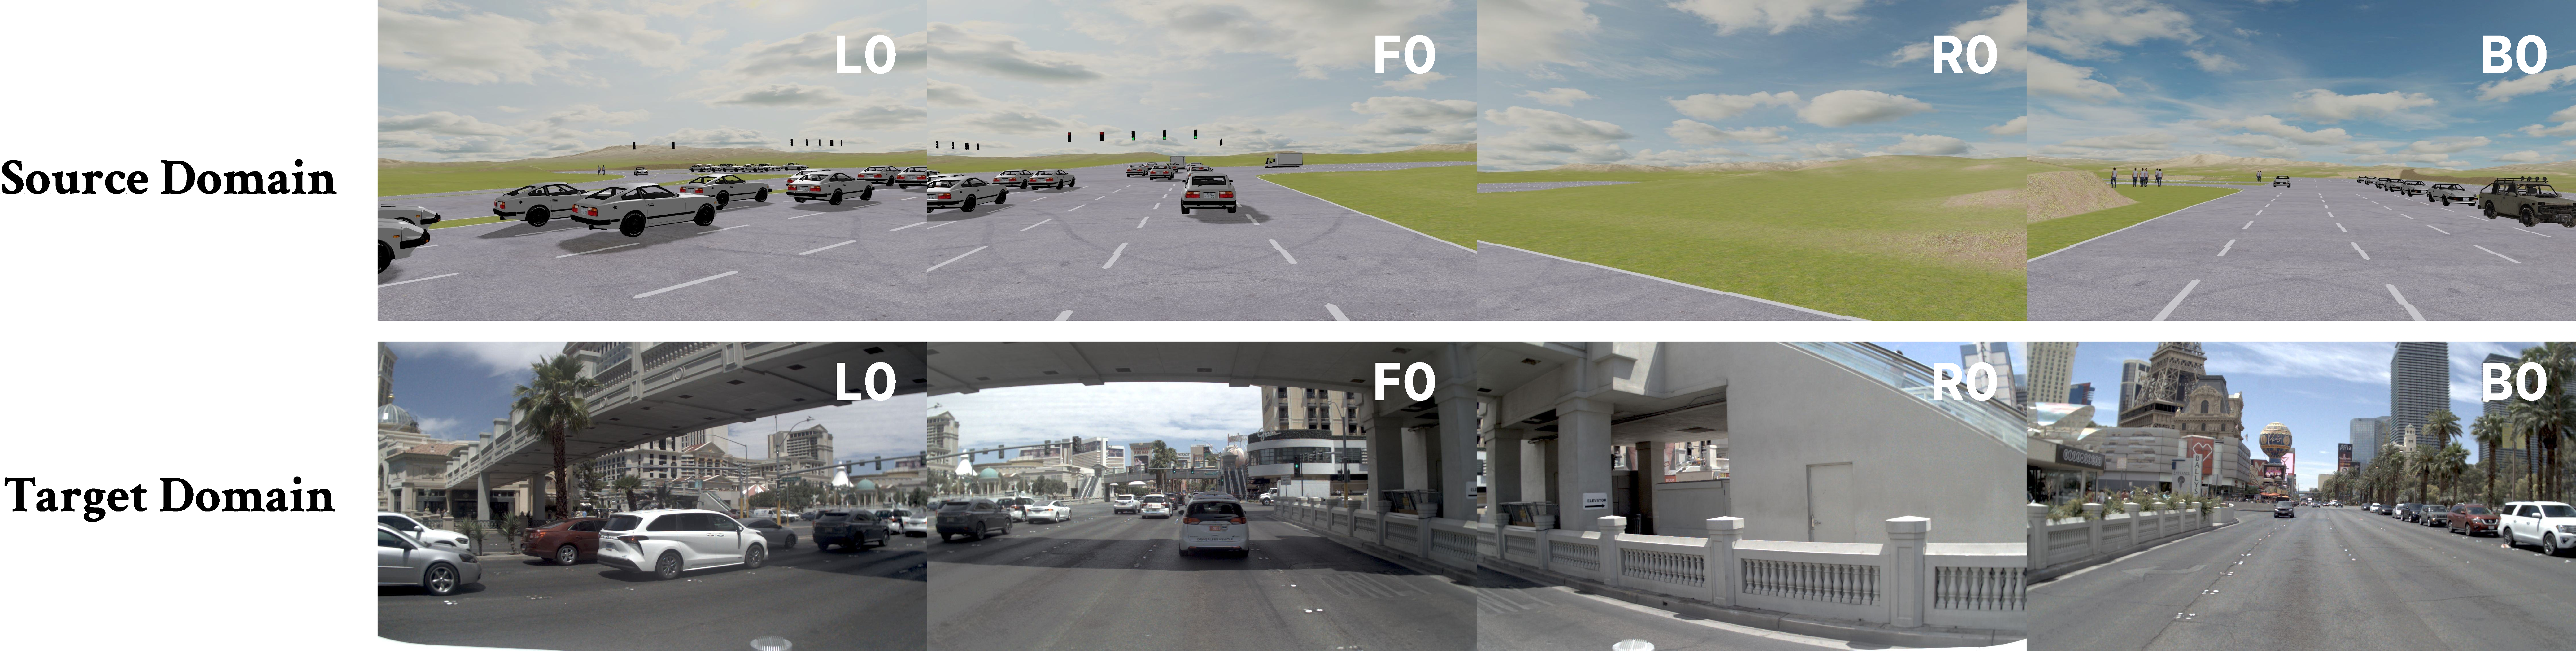
\includegraphics[width=0.95\textwidth]{figs/Appendix_C1.pdf}
  \vspace{-1em}
  \caption{源域与目标域中观测对的示意图。}
  \label{fig:image_pairs}
\end{figure}

沿用~\cite{liu2025flowing}，我们使用多目标损失函数优化校准器。除标准流匹配目标外，中间潜在空间 $\mathcal{Z}$ 还通过\textbf{编码器损失}和\textbf{KL散度损失}显式正则化，以保持语义一致性并维持良态的流形。总训练目标为：
\begin{equation}
    \mathcal{L}_{\mathrm{total}} = \mathcal{L}_{\mathrm{FM}} + \lambda_{\mathrm{enc}} \mathcal{L}_{\mathrm{enc}} + \lambda_{\mathrm{KL}} \mathcal{L}_{\mathrm{KL}},
\end{equation}
其中各分量定义如下：

\begin{itemize}
    \item \textbf{流匹配损失（$\mathcal{L}_{\mathrm{FM}}$）：}我们采用线性概率路径学习源域与目标域分布之间的传输映射。损失定义为：
    \begin{equation}
        \mathcal{L}_{\mathrm{FM}}(\theta) = \mathbb{E}_{t, q(z_t|z_0, z_1)} \left[ \| v_\theta(z_t, t) - (z_1 - z_0) \|^2 \right],
    \end{equation}
    其中 $z_0 \sim \mathcal{D}_{\mathrm{source}}$，$z_1 \sim \mathcal{D}_{\mathrm{target}}$。

    \item \textbf{编码器损失（$\mathcal{L}_{\mathrm{enc}}$）：}我们在源域与目标域特征对之间采用类别对比损失来正则化小型编码器。该项确保对应相似底层状态的潜在特征聚集在一起，同时将不同状态推离。这防止了传输过程中的模式坍缩，并保留了下游策略 $\pi_\phi$ 所需的潜在空间判别结构。

    \item \textbf{KL损失（$\mathcal{L}_{\mathrm{KL}}$）：}为维持结构化且平滑的潜在流形，我们施加相对于标准正态先验 $\mathcal{P}(z) = \mathcal{N}(0, \mathbf{I})$ 的KL散度惩罚：
    \begin{equation}
        \mathcal{L}_{\mathrm{KL}} = D_{\mathrm{KL}}(q(z|o) \,\|\, \mathcal{P}(z)).
    \end{equation}
    这种变分正则化确保流匹配轨迹保持在潜在空间 $\mathcal{Z}$ 的良态区域内。
\end{itemize}

训练期间，我们使用 AdamW~\cite{kingma2014adam} 优化器，学习率为 $1 \times 10^{-4}$，权重衰减为 $0.01$。测试时，通过一阶欧拉求解器对学到的常微分方程（ODE）从 $t=0$ 到 $t=1$ 积分，获得校准后的表征。

\subsection{测试时策略自适应的更多实现细节}
\label{appendix:test-time-adaptation}

为实现第~\ref{subsubsec:intrinsic_q_estimation}~节定义的截断动作值估计器，我们采用蒙特卡洛采样在时域 $H$ 上生成并评估未来的候选展开。经验奖励函数 $R_k(s_t, \mathbf{a}_t)$ 通过计算 \textbf{EPDMS} 来评估每个候选前缀。基于附录~\ref{appendix:eval_metrics} 中建立的子得分定义，我们详细说明在实时闭环执行中实现其精确与估计评估的计算机制。

前缀奖励在数学上被形式化为连续质量特征（$\mathcal{F}$）的选通求和，严格以关键约束（$\mathcal{C}$）的满足为条件：
\begin{equation}
    R_k(s_t, \mathbf{a}_t) = \mathbb{I}_{\mathcal{C}} \cdot \sum_{f \in \mathcal{F}} w_f f(s_{t:t+k}, \mathbf{a}_{t:t+k})
\end{equation}
其中 $\mathbb{I}_{\mathcal{C}} \in \{0, 1\}$ 作为硬安全过滤器。如果候选轨迹违反任何关键约束，则 $\mathbb{I}_{\mathcal{C}} = 0$，该轨迹的期望值立即被清零。

\textbf{运动学舒适度。}由于测试时自适应机制直接作用于时空规划，我们可以显式访问自车的历史状态和预测的未来路径点。因此，我们无需依赖转移近似；通过直接从路径点序列中提取高频运动学导数（加速度、急动度和偏航率），可以确定性地计算精确的舒适度得分。

\textbf{语义与地图感知。}评估依赖地图的指标（如可行驶区域合规（\textbf{DAC}）、行驶方向合规（\textbf{DDC}）、信号灯合规（\textbf{TLC}）和车道保持（\textbf{LK}））需要将生成的路径点锚定到环境拓扑中。为此，我们假设可以访问准确的定位模型和稳健的建图模型，如高精地图（HD Map）或其他在线地图生成模型。候选自车多边形 $\mathcal{P}_{ego}$ 在每个时间步投影，并对照生成的实时语义布局进行几何查询，以计算约束满足度和路线效率。

\textbf{动态安全估计。}评估交互安全性，特别是无过错碰撞（\textbf{NC}）和碰撞时间（\textbf{TTC}），需要预测其他参与者的随机未来。我们假设可以访问周围智能体当前估计的速度和加速度轮廓。利用这些轮廓，我们在规划时域上运动学传播其边界框 $\mathcal{P}_{obj}$，以检查与自车轨迹的相交情况并计算碰撞时间余量。

\textbf{二维替代安全度量。}为在复杂驾驶环境中严谨评估与潜在碰撞的时空接近程度，我们采用二维替代安全度量（Surrogate Safety Measure, SSM）框架。该领域的基础指标是碰撞时间（TTC），它基于投影的碰撞距离（Distance-to-Collision, DTC）评估与冲突的时间接近程度。在评估瞬间的经典恒定速度假设下~\cite{tarko2018surrogate}，基础2D-TTC使用主车 $i$ 与交互智能体 $j$ 之间的相对速度向量 $\boldsymbol{v}_{ij}$ 定义：
\begin{equation}
    TTC = \frac{DTC}{\Vert\boldsymbol{v}_{ij}\Vert}
\end{equation}

虽然计算简单，但标准的恒定速度假设在动态的真实世界驾驶场景中表现出显著缺陷。具体而言，它无法捕获缓慢而有意识的交互行为，如让行、制动或规避机动，这常常在高阶运动学交互中导致不准确的风险评估~\cite{guo2023modeling, laureshyn2010evaluation}。

为解决这些局限，我们采用修正碰撞时间（Modified Time-To-Collision, MTTC）作为主要安全评估指标。MTTC通过纳入相对加速度向量 $(\boldsymbol{a}_i - \boldsymbol{a}_j)$ 放宽恒定速度约束，从而产生更高保真度的二阶时间投影。通过求解运动学位移方程，MTTC的形式化为：
\begin{equation}
    MTTC = \frac{-\Vert\boldsymbol{v}_{ij}\Vert \pm \sqrt{\Vert\boldsymbol{v}_{ij}\Vert^2 + 2(\boldsymbol{a}_i - \boldsymbol{a}_j)DTC}}{\boldsymbol{a}_i - \boldsymbol{a}_j}
\end{equation}
与既定的碰撞预警逻辑一致，最终MTTC通过从该二次公式中提取最小正实根来确定。此外，通过将车辆状态组织为矩阵，我们可以在所有 $i,j$ 对上同时并行计算MTTC。生成的指标集随后根据 Ozbay 等人~\cite{ozbay2008derivation} 确立的行为阈值进行过滤，确保大规模多智能体评估中高保真的风险评估和计算效率。

\section{更多实验细节}

\subsection{闭环评估设置}
\label{appendix:cl_eval_details}
\textbf{场景描述。}我们将三个真实世界数据集转换到BridgeSim平台。\textbf{BridgeSim-NavHard} 源自NAVSIM基准~\cite{navsimv1}，其日志来自以2~Hz记录的 nuPlan 数据集~\cite{caesar2021nuplan}。智能体轨迹通过线性插值上采样到10~Hz，高精地图从nuPlan地图API提取，并带有大空间缓冲区以覆盖完整的自车轨迹。转换后的场景包含421个场景。\textbf{BridgeSim-WOMD} 由 Waymo 开放运动数据集~\cite{ettinger2021large} 转换而来，该数据集以10~Hz在世界坐标系中提供9秒场景。所有智能体和地图位置以自车的初始位置重新居中，自车速度旋转到车辆局部坐标系。转换后的场景包含400个场景。\textbf{BridgeSim-nuScenes} 基于 nuScenes 数据集~\cite{caesar2020nuscenes} 构建，该数据集以2~Hz运行。转换后的场景包含143个场景。相机图像在MetaDrive中以10~Hz重新渲染，每隔五步采样一次以匹配原始关键帧速率。
%\textbf{BridgeSim-Bench2Drive} is derived from CARLA-simulated scenarios in Bench2Drive~\cite{jia2024bench2drive} at 20~Hz. Since CARLA uses a left-handed coordinate system, a handedness flip is applied before conversion. In all cases, the output stores per-agent state arrays (\textit{position}, \textit{heading}, \textit{velocity}, \textit{dimensions}, \textit{valid}) at a unified 10~Hz, along with vectorized HD map features and per-frame traffic light states, all expressed in a scenario-local right-handed coordinate frame.

\noindent \textbf{仿真设置。}所有模型都在默认时间步（\texttt{sim\_dt=0.1s}）的仿真下进行评估。推理以指定的 \texttt{replan\_rate} 执行，在重规划间隔之间消耗缓存的路径点。在评估开始之前执行初始回放阶段，为智能体提供历史时间缓冲。对于多提议模型，轨迹评分器在一组候选轨迹中选择最终规划。对于运行TTA模块，应用观测校准模块，通过固定采样步数的流匹配网络减少仿真与真实世界训练数据之间的域差距。


\subsection{第~\ref{subsec:observational_shift}~节实证研究的细节}
\label{appendix:observational_shift_details}

在第~\ref{subsec:observational_shift}~节的图~\ref{fig:empirical_observational_shift} 中，平均位移误差（Average Displacement Error, ADE）对比是通过在 $4\text{-second}$ 时域上评估策略预测轨迹与真值专家演示的偏差获得的。为量化考虑多模态输出的预测精度，我们通过评估最接近真值的预测轨迹候选来计算最小平均位移误差（$\text{minADE}$）。设 $T$ 为预测时域，$K$ 为预测轨迹候选数，$\mathbf{p}_t$ 为时间步 $t$ 的真值空间坐标，$\hat{\mathbf{p}}_t^{(k)}$ 为第 $k$ 个候选的预测坐标。该指标的形式化为：
\begin{equation}
\small
    \text{minADE} = \min_{k \in \{1, \dots, K\}} \frac{1}{T} \sum_{t=1}^{T} \left\| \hat{\mathbf{p}}_t^{(k)} - \mathbf{p}_t \right\|_2,
\end{equation}
其中 $\| \cdot \|_2$ 表示欧几里得（$L_2$）范数。此外，闭环性能指标使用 \textit{BridgeSim 驾驶得分}在BridgeSim-NavHard场景上进行评估。

\subsection{第~\ref{subsec:objective_mismatch}~节实证研究的细节}
\label{appendix:objective_mismatch_details}

在图~\ref{fig:empirical_objective_mismatch} 所示的分析中，我们使用 \textit{BridgeSim 驾驶得分}作为回报目标 $J(\pi)$ 的实证实现。为确保严谨的评估，我们评估具有代表性的最先进端到端策略家族~\cite{transfuser, diffusiondrive, diffusiondrivev2, RAP, DrivoR}，并报告性能上下界以刻画不同架构范式之间的方差。实验协议定义如下：
\begin{itemize}
    \item 图~\ref{fig:empirical_objective_mismatch}(a)：我们在BridgeSim-NavHard中固定仿真时域 $T=80$ 下评估策略。为隔离执行时域 $k$ 的影响，我们将固定 $k$ 步前缀的基线与通过对策略预测轨迹集穷举搜索得到的“最优执行”基线进行比较。
    \item 图~\ref{fig:empirical_objective_mismatch}(b)：我们在BridgeSim-Navhard中对比两种不同选择标准下策略的性能：1) \textbf{开环目标}，依赖智能体学到的Q值估计器；2) \textbf{闭环目标}，通过真值EPDMS指标选择动作以模拟无偏价值函数。评估在（$T \in \{40, 80, 120, 160\}$）上进行。
    \item 图~\ref{fig:empirical_objective_mismatch}(c)：我们计算各策略开环与闭环指标之间的皮尔逊相关系数。开环指标通过按照NAVSIMV2协议~\cite{navsimv2} 在BridgeSim-NavHard中进行非反应式仿真（$T=40$）获得。相比之下，闭环指标来自BridgeSim-NavHard中不断扩展的仿真时域（$T \in \{40, 80, 120, 160\}$）上的BridgeSim驾驶得分，以观察预测有效性随时间衰减的情况。
\end{itemize}

\begin{figure}[tbh]
  \centering
  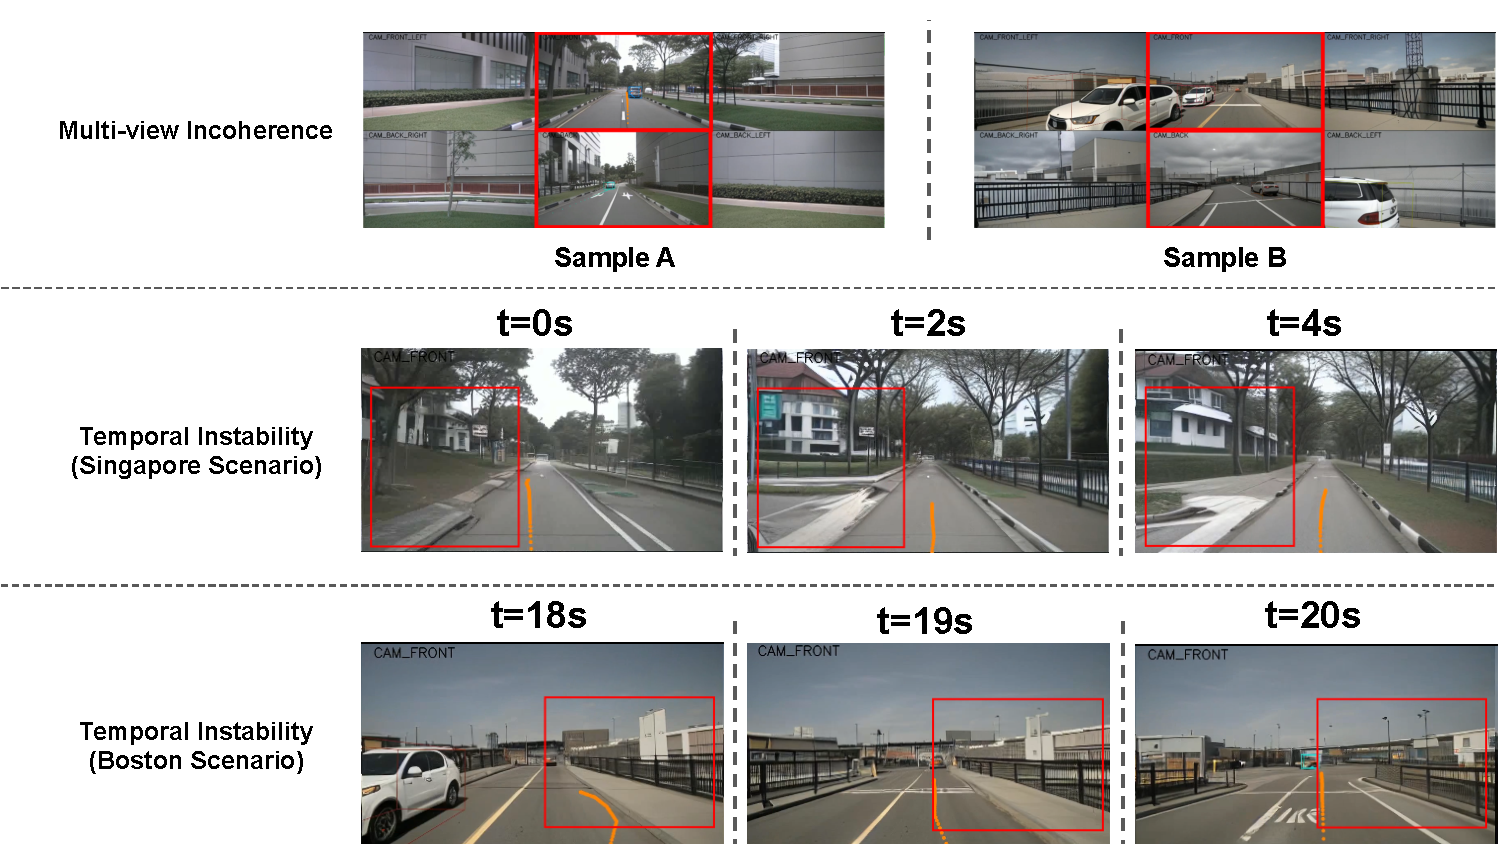
\includegraphics[width=0.95\textwidth]{figs/Appendix_E1.pdf}
  \vspace{-1em}
  \caption{DriveArena中仿真伪影的定性分析：多视图不一致（左）和时间不稳定（右）。红框标出导致策略失败或指标失真的不一致之处。}
  \label{fig:drivearena_artifacts}
\end{figure}

\begin{figure}[tbh]
  \centering
  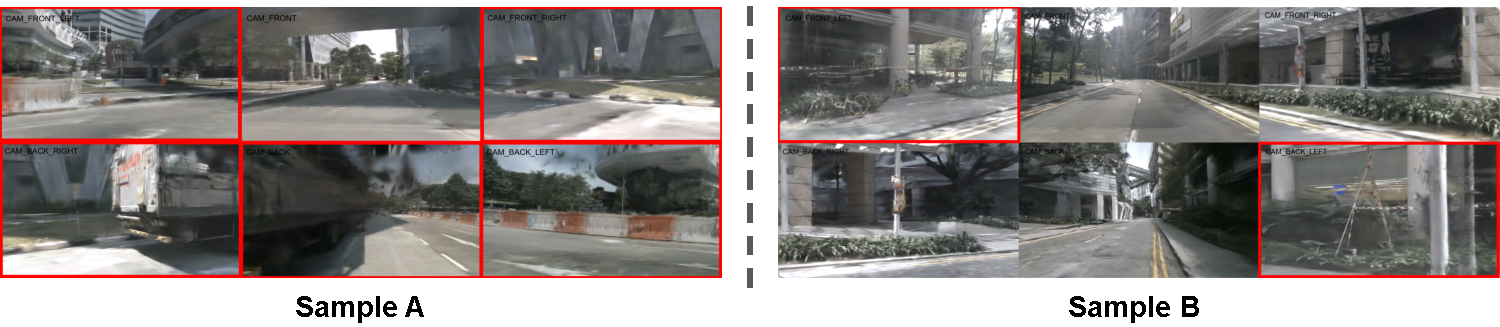
\includegraphics[width=0.95\textwidth]{figs/Appendix_E2.pdf}
  \vspace{-1em}
  \caption{HUGSIM中重建伪影与重影效应的定性分析。红框标出不一致之处。 }
  \label{fig:hugsim_artifacts}
\end{figure}

\begin{table}[tbh]
\centering
\caption{不同反应式交通模式下含完整子指标得分的性能对比。 }
\label{tab:complete_reactive_cl_scores}
\renewcommand{\arraystretch}{1.5}
\setlength{\aboverulesep}{0pt}
\setlength{\belowrulesep}{0pt}
\resizebox{\textwidth}{!}{
\begin{tabular}{l *{11}{c} @{\hspace{6pt} } *{11}{c}}
\toprule
\multirow{2}{*}{\textbf{模型}} & \multicolumn{11}{c}{\textbf{IDM}} & \multicolumn{11}{c}{\textbf{安全关键}} \\
\cmidrule(lr){2-12} \cmidrule(lr){13-23}
& \textbf{DS} & \textbf{EPDMS} & \textbf{RC} & \textbf{NC} & \textbf{DAC} & \textbf{DDC} & \textbf{TL} & \textbf{TTC} & \textbf{LK} & \textbf{HC} & \textbf{EC} & \textbf{DS} & \textbf{EPDM} & \textbf{RC} & \textbf{NC} & \textbf{DAC} & \textbf{DDC} & \textbf{TL} & \textbf{TTC} & \textbf{LK} & \textbf{HC} & \textbf{EC} \\
\midrule
DiffusionDrive & 45.30 & 72.95 & 59.93 & 95.41 & 85.47 & \textbf{100.00} & 98.36 & 89.73 & 89.83 & 92.31 & 40.82 & 38.68 & 68.16 & 54.77 & 93.62 & 83.86 & \textbf{100.00} & 98.36 & 84.97 & 90.71 & 89.56 & 39.13 \\
DiffusionDriveV2 & 31.94 & 65.43 & 45.85 & 94.57 & 82.09 & \textbf{100.00} & 98.23 & 89.10 & 85.42 & 74.52 & 22.99 & 28.17 & 61.45 & 43.50 & 93.15 & 80.78 & \textbf{100.00} & 98.30 & 85.72 & 85.81 & 70.99 & 21.68 \\
RAP & 60.02 & 76.85 & 77.20 & 97.68 & 88.84 & \textbf{100.00} & 98.49 & 93.07 & 78.16 & \textbf{94.49} & \textbf{53.84} & 51.83 & 70.88 & 71.22 & 95.03 & 88.16 & \textbf{100.00} & 98.58 & 86.37 & 78.26 & \textbf{90.22} & \textbf{50.53} \\
\midrule
\rowcolor{green!15} TTA \scriptsize (DiffusionDrive) & 62.68 \scriptsize \textcolor{red}{+17.4} & 84.36 & 72.28 & 96.85 & 95.63 & \textbf{100.00} & 98.98 & 91.57 & \textbf{92.43} & 87.95 & 40.13 & 55.02 \scriptsize \textcolor{red}{+16.3} & 78.95 & 67.92 & 94.73 & 95.21 & \textbf{100.00} & 98.76 & 86.64 & \textbf{91.30} & 83.65 & 37.11 \\
\rowcolor{green!15} TTA \scriptsize (DiffusionDriveV2) & 53.96 \scriptsize \textcolor{red}{+22.0} & 77.47 & 67.89 & 96.08 & 90.53 & \textbf{100.00} & \textbf{99.43} & 89.46 & 89.98 & 85.46 & 29.90 & 47.64 \scriptsize \textcolor{red}{+19.5} & 71.66 & 65.91 & 93.54 & 89.16 & \textbf{100.00} & 99.07 & 84.23 & 90.11 & 81.73 & 27.49 \\
\rowcolor{green!15} TTA \scriptsize (RAP) & \textbf{79.07} \scriptsize \textcolor{red}{+19.1} & \textbf{90.92} & \textbf{86.21} & \textbf{98.28} & \textbf{98.62} & \textbf{100.00} & 99.02 & \textbf{95.31} & 91.52 & 92.60 & 51.38 & \textbf{65.94} \scriptsize \textcolor{red}{+14.1} & \textbf{82.01} & \textbf{78.66} & \textbf{95.30} & \textbf{96.19} & \textbf{100.00} & \textbf{99.14} & \textbf{87.71} & 90.26 & 88.18 & 48.07 \\
\bottomrule
\end{tabular}
}
\end{table}

\subsection{反应式评估实验结果细节}
\label{appendix:detailed_reactive_metrics}
我们在表~\ref{tab:complete_reactive_cl_scores} 中展示反应式评估结果（见表~\ref{tab:reactive_cl_scores}）的完整子指标得分。

\subsection{关于OL训练与评估的更多讨论}
\label{subsec:discussions}
\textbf{在开环代理奖励上进行RL微调会有益于闭环性能吗？}近期论文~\cite{diffusiondrivev2, zhou2025autovla} 主张使用RL微调来提升规划性能，主要利用开环代理奖励作为训练目标。然而，如表~\ref{tab:reactive_cl_scores} 所示，我们对DiffusionDrive和DiffusionDriveV2的比较揭示了开环与闭环结果之间的显著差异。具体而言，DiffusionDriveV2在NAVSIM中取得更高的开环指标，但在闭环仿真中表现出明显的性能下降。这表明优化开环目标并不能保证优化闭环目标。

\textbf{我们在多大程度上可以依赖开环指标预测闭环性能？}图~\ref{fig:empirical_objective_mismatch}(c) 表明，虽然开环指标在短时域（$T=H$）内保持预测有效性，但随着 $T$ 超过 $H$，这种相关性迅速衰减。这种衰减趋势表明，虽然高开环得分意味着策略在分布内场景中具有足够的局部规划熟练度和安全性，但它们在反应式或分布外环境中不能作为闭环性能的可靠预测指标。这些发现提出两个关键结论：1) 扩展开环训练数据在统计上并不能保证闭环性能的提升；2) 有效的策略必须优先采用近似标准Q值估计的目标，以确保长时域稳定性。

\section{现有E2E闭环基准的局限}
\label{appendix:current_e2e_bottlenecks}

现有端到端闭环基准，如 DriveArena~\cite{yang2024drivearena} 和 HUGSIM~\cite{zhou2024hugsim}，表现出源于仿真期间\textit{时间与语义不一致}的局限。

\textbf{DriveArena中的生成式伪影。}
如图~\ref{fig:drivearena_artifacts} 所示，DriveArena表现出显著的仿真差异。\textit{1) 多视图不一致：}在多视图对比中，前后相机视图之间车道标线的颜色、长度和位置差异（红框）可能因观测矛盾而导致策略行为振荡。\textit{2) 时间不稳定：}如时间序列所示，交叉口等道路特征在连续时间戳之间渲染不一致或被自发修改（例如新加坡的 $t=2s$ 和波士顿的 $t=19s$，红框标出），导致场景几何不稳定。

\textbf{HUGSIM中的语义错配。}
如图~\ref{fig:hugsim_artifacts} 所示，HUGSIM等基于3D高斯泼溅的方法在动态参与者集成方面遇到挑战。样本A和B突出显示了移动车辆周围的仿真伪影和模糊（红框），这些经常被误判为障碍物。此外，视觉渲染与底层高精地图之间的错位造成语义不一致。

\textbf{BridgeSim中的结构不变性。}
相比之下，BridgeSim通过将车辆动力学与视觉渲染解耦，保持严格的结构不变性。通过利用MetaDrive物理引擎，运动学状态 $s_t$ 作为环境的确定性参考。传感器观测 $o_t$ 通过几何投影而非生成式合成产生，确保所有相机帧和时间戳上的空间与时间一致性。

\section{未来工作}
我们期待未来研究将聚焦于构建更现实的评估，并开发在真实世界约束下增强驾驶智能体安全性和鲁棒性的方法：

\textbf{1. 端到端闭环基准。}现有闭环基准仍然受限于观测保真度、时间不一致和评估效率（见附录~\ref{appendix:current_e2e_bottlenecks}）。未来基准应转向统一的混合引擎框架，将游戏引擎仿真的可控性与数据驱动世界模型的多样性相结合，实现长时域闭环仿真可扩展且现实的压力测试。

\textbf{2. 端到端闭环训练。}当前开环预训练方法缺乏错误恢复样本和反馈驱动的学习目标，无法教会策略安全地在动态、反应式环境中导航。推进闭环训练方法仍然至关重要，如 RoAD~\cite{garcia2025road} 的可扩展变体、基于世界模型的学习，以及具有可靠奖励公式的强化学习。特别是，在真实世界驾驶中定义和学习反映真实闭环回报的无偏价值函数，是一个关键开放挑战。

\end{document}
